\documentclass{article}

\usepackage{amsmath,amsfonts,latexsym,graphicx}
\usepackage{fullpage,color}
\usepackage{setspace}
\usepackage{float}

\usepackage{tocloft}
\setlength{\cftbeforesecskip}{10pt}
\renewcommand{\cftbeforesubsecskip}{4pt}
\renewcommand{\cftbeforesubsubsecskip}{4pt}
\renewcommand\cftdotsep{2}
\setcounter{secnumdepth}{4}
\setcounter{tocdepth}{4}

\usepackage{fancyhdr}
\usepackage{hyperref}

\usepackage{xeCJK}

\usepackage{indentfirst}
\setlength{\parindent}{2em}

\usepackage[linesnumbered,boxed,ruled,vlined]{algorithm2e}

\usepackage{textgreek}

\usepackage{longtable}

\begin{document}
\begin{titlepage}
\fancyhead[CH]{}

\hspace{3.0cm}
\begin{center}
\vfill
% Upper part of the page

\textsc{\LARGE Tsinghua University}\\[1.5cm]

\textsc{\Large Computer Organization Experimentation}\\[0.5cm]


% Title
\rule[0.75\baselineskip]{0.75\textwidth}{1pt}

{ \huge \bfseries Design Description}\\[0.4cm]

\rule[20\baselineskip]{0.75\textwidth}{1pt}

% Author and supervisor
\begin{minipage}{0.4\textwidth}
\begin{flushleft} \large
\emph{Author:}\\
Shizhi \textsc{Tang}

Xihang \textsc{Liu}

Zixi \textsc{Cai}
\end{flushleft}
\end{minipage}
\begin{minipage}{0.4\textwidth}
\begin{flushright} \large
\emph{Supervisor:} \\
Yuxiang \textsc{Zhang}

Prof.~Weidong \textsc{Liu}
\end{flushright}
\end{minipage}

\vfill
\vspace{3.0cm}
% Bottom of the page
{\large \today}

\end{center}

\end{titlepage}
\setcounter{page}{2}
\tableofcontents
\newpage
\begin{spacing}{1.4}

%%%%%%%%%%%%%%%%%%%%%%
%     BODY BEGIN     %
%%%%%%%%%%%%%%%%%%%%%%

\section{概述}

本文是MIPS32 CPU设计nCore的设计文档。

\subsection{常量}

本文中所使用的常量定义如Table~\ref{tb:constants}。
\begin{table}[!htb]
\begin{center}
\begin{tabular*}{15cm}{l|l|p{10cm}}  
\hline  
\textbf{常量}&\textbf{值}&\textbf{功能} \\
\hline InstWidth            & 31..0    & 指令宽度 \\
\hline DataWidth            & 31..0    & 数据宽度 \\
\hline AddrWidth            & 31..0    & 地址宽度 \\
\hline RegAddrWidth         & 4..0     & 寄存器地址宽度 \\
\hline StallWidth           & 5..0     & 暂停信号宽度,每个分量对应一个需要被暂停的客体 \\
\hline CP0RegAddrWidth      & 4..0     & CP0寄存器地址宽度(仅可容纳nCore实现了的部分寄存器) \\
\hline ExceptionCauseWidth  & 4..0     & 异常编号的宽度 \\
\hline IntWidth             & 5..0     & 外设中断编号宽度 \\
\hline TLBIndexWidth        & 3..0     & TLB表项索引宽度 \\
\hline 
\end{tabular*}  
\caption{常量}
\label{tb:constants}
\end{center}
\end{table}

\subsection{文档结构}

本文按以下结构组织:首先介绍整体的层次划分。对于每一层次,介绍其实体\footnote{实体即VHDL中的entity或Verilog中的module}划分,然后依次介绍各实体。对于每个实体,分别介绍其功能、参数\footnote{参数即VHDL中的generic或Verilog中的parameter,是编译期确定的,用于方便地生成用于不同环境,例如功能测例、\textmu Core和u-boot,的目标逻辑}(如有)、接口和具体设计。

\section{层次划分}

nCore自底向上分为三个层次:数据通路、访存控制和I/O。数据通路层是nCore的核心,此层实现了标准的MIPS五级流水线和CP0协处理器,及其所需的数据旁路、暂停、异常等机制的控制逻辑。访存控制层解决了指令访存和数据访存的结构冲突,将其封装为统一的访存逻辑。I/O层则将统一的访存按不同外设的性质特化。这三层间的数据流关系见Figure~\ref{fig:layer-data-flow}。

\begin{figure}[!htb]
	\centering
	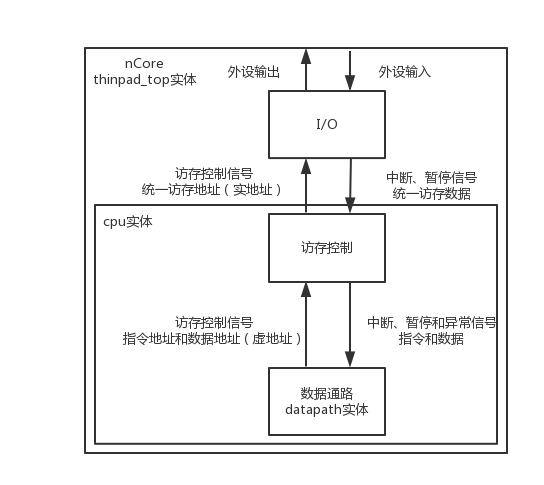
\includegraphics[width=.7\textwidth]{layer-data-flow.png}
	\caption{各层次间的数据流}
    \label{fig:layer-data-flow}
\end{figure}

各层次用组合(Composition)的方式例化,下层实体例化与上层实体中。具体地,数据通路层实现于datapath实体中;访存控制实现于cpu实体中,但cpu实体中也例化了datapath实体;I/O实现于thinpad\_top实体中,但thinpad\_top实体中也例化了cpu实体。像这样将下层实体直接例化在上层实体中,而不是在顶层实体中连接所有层,减少了层间的冗余连接,也对下层实体进行了很好的封装。

下文将依次介绍各个层次。此外,少数实体在逻辑上不属于这三层中的任意一层,例如时钟驱动器,但在实现中例化于某一层的顶层实体中,也将于该层一并介绍。

\section{数据通路层}

\subsection{概述}

数据通路层以MIPS五级流水线为核心。实体id、ex、mem分别实现了译码、执行、访存阶段,实体if\_id、id\_ex、ex\_mem、mem\_wb分别实现了取指/译码、译码/执行、执行/访存、访存/写回间的阶段寄存器。取指和写回阶段不实现于单独的实体:取指逻辑主要实现于程序计数器(PC)实体;写回逻辑由被写入的目标处理,这些目标包括寄存器堆、CP0协处理器、乘除法HI/LO寄存器。实体ctrl通过控制各阶段寄存器实现流水线的暂停和清空(处理异常时)。此外,除法逻辑实现于单独的实体。

本层包含的所有实体见Table~\ref{tb:datapath-entities}:

\begin{table}[!htb]
\begin{center}
\begin{tabular}{p{7.5cm}|p{7.5cm}}  
\hline  
\textbf{实体}&\textbf{功能} \\
\hline datapath & 顶层实体 \\
\hline pc\_reg & 程序计数器(PC) \\
\hline if\_id & 取指/译码阶段寄存器 \\
\hline regfile & 通用寄存器堆 \\
\hline id & 译码阶段 \\
\hline id\_ex & 译码/执行阶段寄存器 \\
\hline ex & 执行阶段 \\
\hline div & 除法器 \\
\hline ex\_mem & 执行/访存阶段寄存器 \\
\hline mem & 访存阶段 \\
\hline mem\_wb & 访存/写回阶段寄存器 \\
\hline hi\_lo & 乘除法HI/LO寄存器 \\
\hline ctrl & 流水线控制器 \\
\hline cp0\_reg & CP0协处理器 \\
\hline 
\end{tabular}  
\caption{数据通路层的实体}
\label{tb:datapath-entities}
\end{center}
\end{table}

\subsection{整体设计}

正常情况下,数据沿流水线逐级传递并加工。数据通路层各实体间的主要数据流见Figure~\ref{fig:datapath-data-flow},其中实线表示正常数据流,虚线表示旁路数据流。

\begin{figure}[!htb]
	\centering
	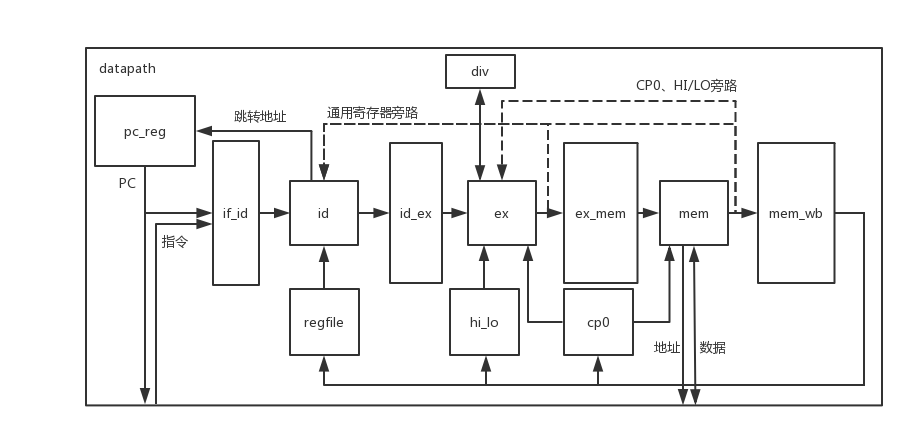
\includegraphics[width=\textwidth]{datapath-data-flow.png}
	\caption{数据通路层数据流}
    \label{fig:datapath-data-flow}
\end{figure}

当有异常发生时,每个阶段将该阶段发生的异常逐级传递至访存阶段。访存阶段根据CP0控制信息向ctrl实体发出异常请求,ctrl实体命令各阶段寄存器进行清空,并修改PC以跳转至异常处理向量。异常处理的控制流见Figure~\ref{fig:datapath-exception-flow}。

\begin{figure}[!htb]
	\centering
	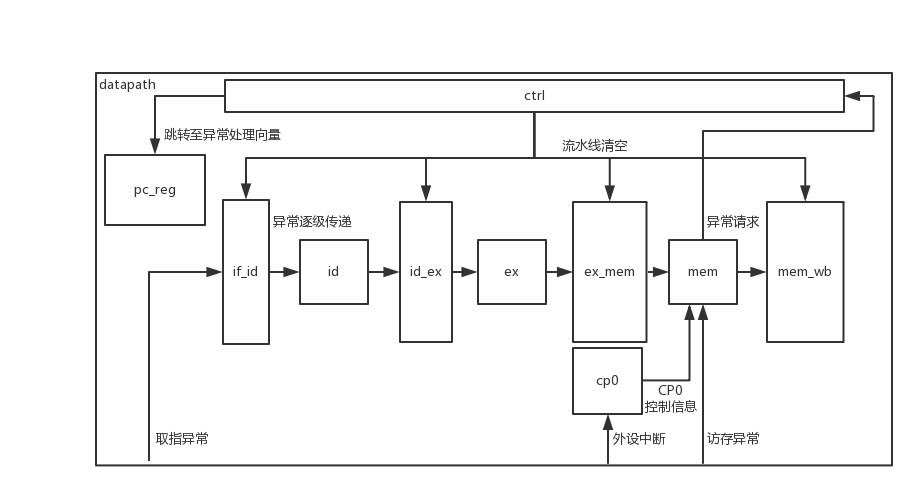
\includegraphics[width=\textwidth]{datapath-exception-flow.png}
	\caption{异常控制流}
    \label{fig:datapath-exception-flow}
\end{figure}

当需要流水线暂停(插入空泡)时,需要暂停的主体向ctrl实体发出暂停请求,ctrl实体命令各阶段寄存器进行暂停。暂停控制流见Figure~\ref{fig:datapath-stall-flow}。

\begin{figure}[!htb]
	\centering
	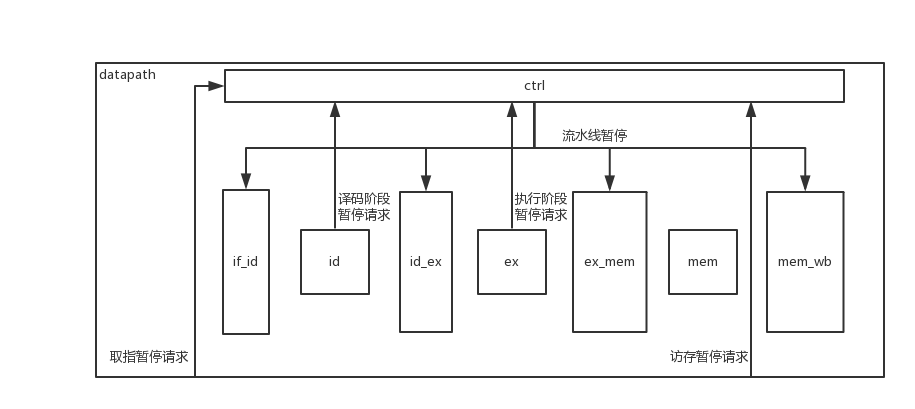
\includegraphics[width=\textwidth]{datapath-stall-flow.png}
	\caption{暂停控制流}
    \label{fig:datapath-stall-flow}
\end{figure}

\subsection{各实体说明}

以下介绍除数据通路层除顶层实体外的各实体。顶层实体datapath的说明见上层(访存控制层)。

\subsubsection{pc\_reg}

\paragraph{功能}\mbox{}

pc\_reg实现了程序计数器(PC)的寄存器。PC中储存了当前处于取指阶段指令的地址。每个周期PC会发生改变,根据pc\_reg的输入,改变分为顺序执行、分支/跳转、异常跳转三种情况。

\paragraph{参数}\mbox{}

pc\_reg实体的参数定义见Table~\ref{tb:pcreg-parameter}。
\begin{table}[!htb]
\begin{center}
\begin{tabular*}{15cm}{l|l|l}  
\hline  
\textbf{参数}&\textbf{类型}&\textbf{功能} \\
\hline instEntranceAddr        & std\_logic\_vector(AddrWidth)    & 重置后PC的值 \\
\hline 
\end{tabular*}  
\caption{pc\_reg实体的参数}
\label{tb:pcreg-parameter}
\end{center}
\end{table}

\paragraph{接口}\mbox{}

pc\_reg实体的接口定义见Table~\ref{tb:pcreg-interface}。
\begin{table}[!htb]
\begin{center}
\begin{tabular*}{15cm}{l|l|l|l|p{5cm}}  
\hline  
\textbf{信号}&\textbf{宽度}&\textbf{I/O}&\textbf{来源/去向}&\textbf{功能} \\
\hline rst                     & 1             & I     & 上层          & 同步重置 \\
\hline clk                     & 1             & I     & 上层          & 时钟 \\
\hline stall\_i                & StallWidth    & I     & ctrl          & 对应pc\_reg的分量为高电平表示需要暂停 \\
\hline branchTargetAddress\_i  & AddrWidth     & I     & id            & 跳转目标 \\
\hline branchFlag\_i           & 1             & I     & id            & 高电平表示需要跳转 \\
\hline flush\_i                & 1             & I     & ctrl          & 高电平表示发生了异常 \\
\hline newPc\_i                & AddrWidth     & I     & ctrl          & 异常处理向量 \\
\hline pc\_o                   & AddrWidth     & O     & if\_id, 上层  & PC \\
\hline pcEnable\_o             & 1             & O     & if\_id        & 高电平表示此指令不是空泡 \\
\hline 
\end{tabular*}  
\caption{pc\_reg实体的接口}
\label{tb:pcreg-interface}
\end{center}
\end{table}

\paragraph{设计}\mbox{}

每个时钟上升沿,若发生了异常,则置PC为异常处理向量,否则判断取指阶段是否被暂停。若被暂停,则PC不变;若未被暂停,则判断是否发生了分支/跳转。若是,则置PC为分支/跳转目标,否则置PC为下一条指令地址(PC+4)。

其中,在判断分支/跳转时,正常情况下,表示是否跳转以及跳转目标的信号来自译码阶段。但是若上一个周期取指阶段被暂停了,此周期译码阶段会是空泡,导致接收不到上述信号。故pc\_reg会在取指暂停时依旧接收跳转相关信号并保存之,待恢复执行后使用。

重置时,PC会被置为由参数指定的的程序入口地址。

\subsubsection{if\_id}

\paragraph{功能}\mbox{}

if\_id是取指阶段与译码阶段间的阶段寄存器,用于保存某个周期取指的结果,在下一个周期交予译码阶段。作为阶段寄存器,if\_id会接受ctrl实体的控制。

本实体可能会向流水线引入的新异常有:读入地址无效异常、读入TLB缺失异常。

\paragraph{接口}\mbox{}

if\_id实体的接口定义见Table~\ref{tb:ifid-interface}。
\begin{table}[!htb]
\begin{center}
\begin{tabular*}{15cm}{l|l|l|l|p{5cm}}
\hline
\textbf{信号}&\textbf{宽度}&\textbf{I/O}&\textbf{来源/去向}&\textbf{功能} \\
\hline rst                     & 1                      & I     & 上层          & 同步重置 \\
\hline clk                     & 1                      & I     & 上层          & 时钟 \\
\hline pc\_i                   & AddrWidth              & I     & pc\_reg       & PC \\
\hline instEnable\_i           & 1                      & I     & pc\_reg       & 高电平表示此指令不是空泡 \\
\hline inst\_i                 & InstWidth              & I     & 上层          & 指令 \\
\hline exceptCause\_i          & ExceptionCauseWidth    & I     & 上层          & 取指异常类型或无异常 \\
\hline pc\_o                   & AddrWidth              & O     & id            & PC \\
\hline valid\_o                & 1                      & O     & id            & 高电平表示此指令不是空泡 \\
\hline inst\_o                 & InstWidth              & O     & id            & 指令 \\
\hline exceptCause\_o          & ExceptionCauseWidth    & O     & id            & 取指异常类型或无异常 \\
\hline stall\_i                & StallWidth             & I     & ctrl          & 对应if\_id的分量为高电平表示需要暂停 \\
\hline flush\_i                & 1                      & I     & ctrl          & 高电平表示流水线需要清空 \\
\hline
\end{tabular*}
\caption{if\_id实体的接口}
\label{tb:ifid-interface}
\end{center}
\end{table}

\paragraph{设计}\mbox{}

各阶段寄存器的值在时钟上升沿发生如下变化:若流水线需要清空,或是ctrl实体恰好暂停了取指阶段,却没有暂停后续的译码阶段,则置零/无效信号,因为没有指令可供译码阶段执行;否则,若取值和译码阶段均被暂停,则维持上一个周期的值,以便译码阶段重复执行;再否则,置为来自取指阶段的值,让译码阶段获得新指令。

重置时,各寄存器置零或无效值。

\subsubsection{regfile}

\paragraph{功能}\mbox{}

实现了32个通用寄存器,支持同时进行两路读和一路写操作。

\paragraph{接口}\mbox{}

regfile实体的接口定义见Table~\ref{tb:regfile-interface}。
\begin{table}[!htb]
\begin{center}
\begin{tabular*}{15cm}{l|l|l|l|p{5cm}}
\hline
\textbf{信号}&\textbf{宽度}&\textbf{I/O}&\textbf{来源/去向}&\textbf{功能} \\
\hline rst                     & 1                      & I     & 上层          & 同步重置 \\
\hline clk                     & 1                      & I     & 上层          & 时钟 \\
\hline writeEnable\_i          & 1                      & I     & mem\_wb       & 写入使能 \\
\hline writeAddr\_i            & RegAddrWidth           & I     & mem\_wb       & 写入地址 \\
\hline writeData\_i            & DataWidth              & I     & mem\_wb       & 写入数据 \\
\hline readEnable1\_i          & 1                      & I     & id            & 第一路读出使能 \\
\hline readAddr1\_i            & RegAddrWidth           & I     & id            & 第一路读出地址 \\
\hline readData1\_i            & DataWidth              & O     & id            & 第一路读出数据 \\
\hline readEnable2\_i          & 1                      & I     & id            & 第二路读出使能 \\
\hline readAddr2\_i            & RegAddrWidth           & I     & id            & 第二路读出地址 \\
\hline readData2\_i            & DataWidth              & O     & id            & 第二路读出数据 \\
\hline
\end{tabular*}
\caption{regfile实体的接口}
\label{tb:regfile-interface}
\end{center}
\end{table}

\paragraph{设计}\mbox{}

写入使能时,寄存器的值在时钟上升沿时置为输入的值(时序逻辑)。读出使能时,立即输出当前寄存器的值(组合逻辑)。特殊地,当读出地址与写入地址相同时,输出将要被写入的值(数据旁路)。此外寄存器0的输出永远是0。

重置时所有寄存器将会被置零。

\subsubsection{id}

\paragraph{功能}\mbox{}

本实体实现了MIPS五级流水线的译码阶段。

本实体可能向流水线引入的新异常有:指令无效异常、系统调用、断点异常、ERET(nCore通过MIPS预留的14号异常实现ERET指令)、读入地址无效异常(当分支/跳转目标地址无效时触发)。

\paragraph{接口}\mbox{}

id实体的接口定义见Table~\ref{tb:id-interface}。
\begin{table}[!htb]
\begin{center}
\begin{tabular*}{17cm}{l|l|l|l|p{5cm}}
\hline
\textbf{信号}&\textbf{宽度}&\textbf{I/O}&\textbf{来源/去向}&\textbf{功能} \\
\hline rst                     & 1                      & I     & 上层          & 重置 \\
\hline pc\_i                   & AddrWidth              & I     & if\_id        & 指令地址 \\
\hline inst\_i                 & InstWidth              & I     & if\_id        & 指令 \\
\hline regData1\_i             & DataWidth              & I     & regfile       & 通用寄存器堆的第一路读出数据 \\
\hline regData2\_i             & DataWidth              & I     & regfile       & 通用寄存器堆的第二路读出数据 \\
\hline exToWriteReg\_i         & 1                      & I     & ex            & 自执行阶段旁路的通用寄存器写使能 \\
\hline exToWriteRegAddr\_i     & RegAddrWidth           & I     & ex            & 自执行阶段旁路的通用寄存器写地址 \\
\hline exToWriteRegData\_i     & DataWidth              & I     & ex            & 自执行阶段旁路的通用寄存器写数据 \\
\hline memToWriteReg\_i        & 1                      & I     & ex            & 自访存阶段旁路的通用寄存器写使能 \\
\hline memToWriteRegAddr\_i    & RegAddrWidth           & I     & ex            & 自访存阶段旁路的通用寄存器写地址 \\
\hline memToWriteRegData\_i    & DataWidth              & I     & ex            & 自访存阶段旁路的通用寄存器写数据 \\
\hline toStall\_o              & 1                      & O     & ctrl          & 请求暂停 \\
\hline regReadEnable1\_o       & 1                      & O     & regfile       & 通用寄存器堆的第一路读出使能 \\
\hline regReadEnable2\_o       & 1                      & O     & regfile       & 通用寄存器堆的第二路读出使能 \\
\hline regReadAddr1\_o         & RegAddrWidth           & O     & regfile       & 通用寄存器堆的第一路读出地址 \\
\hline regReadAddr2\_o         & RegAddrWidth           & O     & regfile       & 通用寄存器堆的第二路读出地址 \\
\hline alut\_o                 & 由综合器指定(枚举类型) & O     & id\_ex        & 译码结果:运算器运算类型 \\
\hline memt\_o                 & 由综合器指定(枚举类型) & O     & id\_ex        & 译码结果:访存类型 \\
\hline lastMemt\_i             & 由综合器指定(枚举类型) & I     & id\_ex        & 上一条指令的访存类型,用于判断是否需要暂停 \\
\hline operand1\_o             & DataWidth              & O     & id\_ex        & 译码结果:操作数1 \\
\hline operand2\_o             & DataWidth              & O     & id\_ex        & 译码结果:操作数2 \\
\hline operandX\_o             & DataWidth              & O     & id\_ex        & 译码结果:附加操作数 \\
\hline toWriteReg\_o           & 1                      & O     & id\_ex        & 译码结果:通用寄存器写使能 \\
\hline writeRegAddr\_o         & RegAddrWidth           & O     & id\_ex        & 译码结果:通用寄存器写地址 \\
\hline isInDelaySlot\_i        & 1                      & I     & id\_ex        & 高电平表示本指令在延迟槽内 \\
\hline isInDelaySlot\_o        & 1                      & O     & id\_ex        & 高电平表示本指令在延迟槽内 \\
\hline nextInstInDelaySlot\_o  & 1                      & O     & id\_ex        & 高电平表示下一条指令是延迟槽 \\
\hline branchFlag\_o           & 1                      & O     & pc\_reg       & 分支/跳转使能 \\
\hline branchTargetAddress\_o  & AddrWidth              & O     & pc\_reg       & 分支/跳转地址 \\
\hline linkAddr\_o             & AddrWidth              & O     & id\_ex        & 译码结果:JAL和JALR指令的链接地址 \\
\hline valid\_i                & 1                      & I     & if\_id        & 高电平表示此指令不是空泡 \\
\hline valid\_o                & 1                      & O     & id\_ex        & 高电平表示此指令不是空泡 \\
\hline exceptCause\_i          & ExceptionCauseWidth    & I     & if\_id        & 截至译码阶段前发生的异常类型或无异常 \\
\hline exceptCause\_o          & ExceptionCauseWidth    & O     & id\_ex        & 截至译码阶段后发生的异常类型或无异常 \\
\hline currentInstAddr\_o      & AddrWidth              & O     & id\_ex        & 指令地址 \\
\hline
\end{tabular*}
\caption{id实体的接口}
\label{tb:id-interface}
\end{center}
\end{table}

\paragraph{设计}\mbox{}

id实体是组合逻辑电路,与时钟无关。

id实体的主要功能是译码,即根据指令各个比特的模式得出该指令的操作类型(包括运算器类型、访存类型、是否需要写入寄存器等)和操作数。

解析操作类型的过程直接却繁琐,直接之处在于只需根据MIPS32定义的各指令比特模式判断即可;繁琐在于指令总数众多,而且MIPS32为了节省比特,或出于历史原因,各指令的比特模式并不完全统一。id实体在实现译码时,简单嵌套了若干层VHDL的case语句进行匹配。未通过case语句找到匹配的指令视作无效指令,应抛出异常。值得注意的是,许多指令要求其中某一段或几段比特为全零,为了减少冗余代码,id实体中复用了一个函数zeroJudge专门用于检查此要求。

id实体对于解析操作数的过程则进行了更好的代码复用。虽然不同指令的操作数(形式地址)含义不同,即寻址方式不同,但操作数的含义均为以下两种之一:寄存器地址,或在指令字中不同位置的立即数(依不同情况需进行符号扩展或零扩展)。id实体在解析操作类型时先以并解析出操作数的含义,然后交由专门的逻辑解析操作数的值。若操作数为立即数,则判断其位置及扩展方式,从指令字中解析。若操作数为寄存器地址,则从regfile实体读取,但还应考虑注意数据冲突:如果来自执行阶段旁路的寄存器写入地址与要读取的寄存器地址相同,则应取用来自旁路的值;若来自执行阶段的旁路数据不适用,还应考虑来自访存阶段的旁路数据。然而,对于上一条指令是访存指令的数据冲突,则不能通过数据旁路解决,此时id实体会向ctrl实体申请流水线中截至译码阶段的部分暂停一个周期。

大多数指令只有不多于两个的操作数,对应id实体的前缀为operand1和operand2两组输出信号,这两组输出信号实现了所有上述操作数类型。对于变址寻址的store指令,还需要第三个操作数,此操作数只需实现立即数寻址即可。故id实体将其作为附加操作数输出,即前缀为operandX的一组信号。

id实体还需处理分支/跳转逻辑。若某条指令为分支/跳转指令,id实体会先判断该分支是否有效(或为无条件的跳转),然后向pc\_reg实体输出跳转使能和跳转目标地址。此外,id实体还会判断跳转的目标地址是否为有效地址(指令字长的整数倍的地址),若为无效地址则抛出相应异常。

某些指令是在译码阶段就可以辨别的自陷指令,例如SYSCALL。此外nCore也利用自陷机制来实现ERET指令。对于这类指令,id实体会将相应的异常输出到流水线上。

以上逻辑较为复杂,导致代码中有较长的process。为了代码复用,还引入了若干中间变量和辅助函数。尽管如此,却不必担心影响性能,因为整个id实体是一个组合逻辑电路,VHDL综合器会将其视作一个整体进行优化。

\subsubsection{id\_ex}

\paragraph{功能}\mbox{}

id\_ex是译码阶段与执行阶段间的阶段寄存器,用于保存某个周期译码的结果,在下一个周期交予执行阶段。作为阶段寄存器,id\_ex会接受ctrl实体的控制。

\paragraph{接口}\mbox{}

id\_ex实体的接口定义见Table~\ref{tb:idex-interface}。
\begin{table}[!htb]
\begin{center}
\begin{tabular*}{17cm}{l|l|l|l|p{5cm}}
\hline
\textbf{信号}&\textbf{宽度}&\textbf{I/O}&\textbf{来源/去向}&\textbf{功能} \\
\hline rst                     & 1                      & I     & 上层          & 同步重置 \\
\hline clk                     & 1                      & I     & 上层          & 时钟 \\
\hline stall\_i                & StallWidth             & I     & ctrl          & 对应if\_id的分量为高电平表示需要暂停 \\
\hline flush\_i                & 1                      & I     & ctrl          & 高电平表示流水线需要清空 \\
\hline alut\_i                 & 由综合器指定(枚举类型) & I     & id            & 译码结果:运算器运算类型 \\
\hline memt\_i                 & 由综合器指定(枚举类型) & I     & id            & 译码结果:访存类型 \\
\hline operand1\_i             & DataWidth              & I     & id            & 译码结果:操作数1 \\
\hline operand2\_i             & DataWidth              & I     & id            & 译码结果:操作数2 \\
\hline operandX\_i             & DataWidth              & I     & id            & 译码结果:附加操作数 \\
\hline toWriteReg\_i           & 1                      & I     & id            & 译码结果:通用寄存器写使能 \\
\hline writeRegAddr\_i         & RegAddrWidth           & I     & id            & 译码结果:通用寄存器写地址 \\
\hline idlinkAddresss\_i       & AddrWidth              & I     & id            & 译码结果:JAL和JALR指令的链接地址 \\
\hline idIsInDelaySlot\_i      & 1                      & I     & id            & 高电平表示本指令在延迟槽内 \\
\hline nextInstInDelaySlot\_i  & 1                      & I     & id            & 高电平表示下一条指令是延迟槽 \\
\hline idCurrentInstAddr\_i    & AddrWidth              & I     & id            & 指令地址 \\
\hline idExceptCause\_i        & ExceptionCauseWidth    & I     & id            & 截至译码阶段后的异常类型或无异常 \\
\hline valid\_i                & 1                      & I     & id            & 高电平表示此指令不是空泡 \\
\hline alut\_o                 & 由综合器指定(枚举类型) & O     & ex            & 译码结果:运算器运算类型 \\
\hline memt\_o                 & 由综合器指定(枚举类型) & O     & ex            & 译码结果:访存类型 \\
\hline operand1\_o             & DataWidth              & O     & ex            & 译码结果:操作数1 \\
\hline operand2\_o             & DataWidth              & O     & ex            & 译码结果:操作数2 \\
\hline operandX\_o             & DataWidth              & O     & ex            & 译码结果:附加操作数 \\
\hline toWriteReg\_o           & 1                      & O     & ex            & 译码结果:通用寄存器写使能 \\
\hline writeRegAddr\_o         & RegAddrWidth           & O     & ex            & 译码结果:通用寄存器写地址 \\
\hline exlinkAddress\_o        & AddrWidth              & O     & ex            & 译码结果:JAL和JALR指令的链接地址 \\
\hline exIsInDelaySlot\_o      & 1                      & O     & ex            & 高电平表示本指令(当前在EX阶段的指令)在延迟槽内 \\
\hline isInDelaySlot\_o        & 1                      & O     & id            & 高电平表示本指令(当前在ID阶段的指令)在延迟槽内 \\
\hline exCurrentInstAddr\_o    & AddrWidth              & O     & ex            & 指令地址 \\
\hline exExceptCause\_o        & ExceptionCauseWidth    & O     & ex            & 截至译码阶段后的异常类型或无异常 \\
\hline valid\_o                & 1                      & O     & ex            & 高电平表示此指令不是空泡 \\
\hline
\end{tabular*}
\caption{id\_ex实体的接口}
\label{tb:idex-interface}
\end{center}
\end{table}

\paragraph{设计}\mbox{}

各阶段寄存器的值在时钟上升沿发生如下变化:若流水线需要清空,或是ctrl实体恰好暂停了译码阶段,却没有暂停后续的执行阶段,则置零/无效信号,因为没有指令可供执行阶段执行;否则,若译码和执行阶段均被暂停,则维持上一个周期的值,以便执行阶段重复执行;再否则,置为来自译码阶段的值,让执行阶段获得新指令。

唯一例外的是:isInDelaySlot\_o是用于在下一个周期告知译码阶段“译码阶段中的指令是否在延迟槽中”的,并不传递到下一阶段。当译码阶段被暂停时,不管执行阶段被暂停与否,都应保持上一个周期的值。

重置时,各寄存器置零或无效值。

\subsubsection{ex}

\paragraph{功能}\mbox{}

本实体实现了MIPS五级流水线的执行阶段。对于算数逻辑运算指令,执行阶段负责计算运算结果。对于访存指令(MIPS的访存指令均为变址寻址),执行阶段负责计算访存地址,并将要写入的数据(如有)从译码阶段解析出的操作数传递至访存阶段。对于与HI/LO寄存器或CP0协处理器交互的指令,执行阶段负责解析出比译码阶段更具体的操作类型和操作数。

本实体可能向流水线引入的新异常有:算术溢出异常、读入地址无效异常、输出地址无效异常。

\paragraph{接口}\mbox{}

ex实体的接口定义见Table~\ref{tb:ex-interface}。
\begin{longtable}{l|l|l|l|p{5cm}}
\hline
\textbf{信号}&\textbf{宽度}&\textbf{I/O}&\textbf{来源/去向}&\textbf{功能} \\
\hline \endhead rst            & 1                      & I     & 上层          & 重置 \\
\hline alut\_i                 & 由综合器指定(枚举类型) & I     & id\_ex        & 译码结果:运算器运算类型 \\
\hline memt\_i                 & 由综合器指定(枚举类型) & I     & id\_ex        & 译码结果:访存类型 \\
\hline operand1\_i             & DataWidth              & I     & id\_ex        & 译码结果:操作数1 \\
\hline operand2\_i             & DataWidth              & I     & id\_ex        & 译码结果:操作数2 \\
\hline operandX\_i             & DataWidth              & I     & id\_ex        & 译码结果:附加操作数 \\
\hline toWriteReg\_i           & 1                      & I     & id\_ex        & 译码结果:通用寄存器写使能 \\
\hline writeRegAddr\_i         & RegAddrWidth           & I     & id\_ex        & 译码结果:通用寄存器写地址 \\
\hline linkAddr\_i             & AddrWidth              & I     & id\_ex        & 译码结果:JAL和JALR指令的链接地址 \\
\hline isInDelaySlot\_i        & 1                      & I     & id\_ex        & 高电平表示本指令在延迟槽内 \\
\hline toStall\_o              & 1                      & O     & ctrl          & 请求暂停 \\
\hline toWriteReg\_o           & 1                      & O     & ex\_mem、id   & 译码结果:通用寄存器写使能 \\
\hline writeRegAddr\_o         & RegAddrWidth           & O     & ex\_mem、id   & 译码结果:通用寄存器写地址 \\
\hline writeRegData\_o         & DataWidth              & O     & ex\_mem、id   & 执行结果:通用寄存器写数据 \\
\hline hi\_i                   & DataWidth              & I     & hi\_lo        & 读出HI寄存器的值 \\
\hline lo\_i                   & DataWidth              & I     & hi\_lo        & 读出LO寄存器的值 \\
\hline memToWriteHi\_i         & 1                      & I     & mem           & 访存阶段旁路的HI寄存器写使能 \\
\hline memToWriteLo\_i         & 1                      & I     & mem           & 访存阶段旁路的LO寄存器写使能 \\
\hline memToWriteHiData\_i     & DataWidth              & I     & mem           & 访存阶段旁路的HI寄存器值 \\
\hline memToWriteLoData\_i     & DataWidth              & I     & mem           & 访存阶段旁路的LO寄存器值 \\
\hline wbToWriteHi\_i          & 1                      & I     & mem\_wb       & 写回阶段旁路的HI寄存器写使能 \\
\hline wbToWriteLo\_i          & 1                      & I     & mem\_wb       & 写回阶段旁路的LO寄存器写使能 \\
\hline wbToWriteHiData\_i      & DataWidth              & I     & mem\_wb       & 写回阶段旁路的HI寄存器值 \\
\hline wbToWriteLoData\_i      & DataWidth              & I     & mem\_wb       & 写回阶段旁路的LO寄存器值 \\
\hline toWriteHi\_o            & 1                      & O     & ex\_mem       & 执行结果:写入HI寄存器的使能 \\
\hline toWriteLo\_o            & 1                      & O     & ex\_mem       & 执行结果:写入LO寄存器的使能 \\
\hline writeHiData\_o          & DataWidth              & O     & ex\_mem       & 执行结果:写入HI寄存器的值 \\
\hline writeLoData\_o          & DataWidth              & O     & ex\_mem       & 执行结果:写入LO寄存器的值 \\
\hline memAddr\_o              & AddrWidth              & O     & ex\_mem       & 执行结果:访存地址 \\
\hline memData\_o              & DataWidth              & O     & ex\_mem       & 执行结果:访存写入数据 \\
\hline tempProduct\_i          & 63..0                  & I     & ex\_mem       & 乘法中间结果:部分积 \\
\hline cnt\_i                  & 1..0                   & I     & ex\_mem       & 乘法中间结果:乘加、乘减指令的阶段 \\
\hline tempProduct\_o          & 63..0                  & O     & ex\_mem       & 乘法中间结果:部分积 \\
\hline cnt\_o                  & 1..0                   & O     & ex\_mem       & 乘法中间结果:乘加、乘减指令的阶段 \\
\hline divEnable\_o            & 1                      & O     & div           & 除法器使能 \\
\hline dividend\_o             & DataWidth              & O     & div           & 被除数 \\
\hline divider\_o              & DataWidth              & O     & div           & 除数 \\
\hline divBusy\_i              & 1                      & I     & div           & 高电平表示除法器正忙 \\
\hline quotient\_i             & DataWidth              & I     & div           & 商 \\
\hline remainder\_i            & DataWidth              & I     & div           & 余数 \\
\hline cp0RegReadAddr\_o       & CP0RegAddrWidth        & O     & cp0\_reg      & CP0寄存器读地址 \\
\hline cp0RegData\_i           & DataWidth              & I     & cp0\_reg      & 读出的CP0寄存器值 \\
\hline cp0RegWriteAddr\_o      & CP0RegAddrWidth        & O     & ex\_mem       & 执行结果:CP0寄存器写地址 \\
\hline cp0RegData\_o           & DataWidth              & O     & ex\_mem       & 执行结果:写入的CP0寄存器值 \\
\hline cp0RegWe\_o             & 1                      & O     & ex\_mem       & 执行结果:写入的CP0寄存器使能 \\
\hline memCP0RegWe\_i          & 1                      & I     & mem           & 访存阶段旁路的CP0寄存器写使能 \\
\hline memCP0RegWriteAddr\_i   & CP0RegAddrWidth        & I     & mem           & 访存阶段旁路的CP0寄存器写地址 \\
\hline memCP0RegWriteData\_i   & DataWidth              & I     & mem           & 访存阶段旁路的CP0寄存器写数据 \\
\hline isTlbwi\_o              & 1                      & O     & ex\_mem       & 执行结果:高电平表示本指令是TLBWI \\
\hline isTlbwr\_o              & 1                      & O     & ex\_mem       & 执行结果:高电平表示本指令是TLBWR \\
\hline valid\_i                & 1                      & I     & id\_ex        & 高电平表示此指令不是空泡 \\
\hline valid\_o                & 1                      & O     & ex\_mem       & 高电平表示此指令不是空泡 \\
\hline exceptCause\_i          & ExceptionCauseWidth    & I     & id\_ex        & 截至执行阶段前发生的异常类型或无异常 \\
\hline exceptCause\_o          & ExceptionCauseWidth    & O     & ex\_mem       & 截至执行阶段后发生的异常类型或无异常 \\
\hline currentInstAddr\_i      & AddrWidth              & I     & id\_ex        & 指令地址 \\
\hline currentInstAddr\_o      & AddrWidth              & O     & ex\_mem       & 指令地址 \\
\hline isInDelaySlot\_o        & 1                      & O     & ex\_mem       & 高电平表示本指令在延迟槽内 \\
\hline
\caption{ex实体的接口}
\label{tb:ex-interface}
\end{longtable}

\paragraph{设计}\mbox{}

执行阶段与访存阶段类似,也是纯组合逻辑电路,与时钟无关。其实现逻辑也是根据输入的不同操作类型,对数据进行不同处理。如果操作数来自于HI/LO寄存器或CP0协处理器,也要通过数据旁路解决数据冲突(由于hi\_lo实体未进行旁路处理,关于HI/LO寄存器,需处理来自访存和写回两个阶段的旁路,而对于CP0协处理器,只需处理来自访存的旁路。此处可待日后重构优化)。

乘法、除法、乘加和乘减指令较为复杂,故分多个周期完成。为了解耦合,除法在单独的除法器实体div中完成,而乘法、乘加和乘减在ex实体中完成(日后也可将乘法、乘加和乘减移至单独实体以进一步减少耦合)。为了保持ex实体为纯粹的组合逻辑电路,乘法、乘加和乘减所需的中间状态存储于阶段寄存器ex\_mem实体中:每个周期结束前将中间结果保存在ex\_mem中,待下一个周期开始时再取回。当某条多周期指令还未处理完成时,ex实体会向ctrl实体发出暂停请求,暂停流水线ex及其之前的部分。

ex寄存器可能抛出两类异常。一是某些算术指令要求在溢出时抛出的算术溢出异常;二是变址寻址时若计算出的访存地址无效,需抛出读或写的地址无效异常。

此外,ex实体中求补码、判断溢出的逻辑被使用多次,故复用为函数。

\subsubsection{div}

\paragraph{功能}\mbox{}

独立的除法器。

\paragraph{接口}\mbox{}

div实体的接口定义见Table~\ref{tb:div-interface}。
\begin{table}[!htb]
\begin{center}
\begin{tabular*}{17cm}{l|l|l|l|p{5cm}}
\hline
\textbf{信号}&\textbf{宽度}&\textbf{I/O}&\textbf{来源/去向}&\textbf{功能} \\
\hline clk                     & 1                      & I     & 上层         & 时钟 \\
\hline enable\_i               & 1                      & I     & ex           & 使能 \\
\hline dividend\_i             & DataWidth              & I     & ex           & 被除数 \\
\hline divider\_i              & DataWidth              & I     & ex           & 除数 \\
\hline busy\_o                 & 1                      & O     & ex           & 高电平表示除法器正忙 \\
\hline quotient\_o             & DataWidth              & O     & ex           & 商 \\
\hline remainder\_o            & DataWidth              & O     & ex           & 余数 \\
\hline
\end{tabular*}
\caption{div实体的接口}
\label{tb:div-interface}
\end{center}
\end{table}

\paragraph{设计}\mbox{}

本实体实现了32位除数和被除数的一位原码恢复余数除法器,即需要32个周期完成除法。当运算还未结束时,div实体会通过busy\_o信号告知ex实体等待。若DIV指令的操作数为负数,需在ex实体先转换成原码再进行计算,最后再于ex实体将商和余数转换回补码。

\subsubsection{ex\_mem}

\paragraph{功能}\mbox{}

ex\_mem是执行阶段与访存阶段间的阶段寄存器,用于保存某个周期执行的结果,在下一个周期交予访存阶段。作为阶段寄存器,ex\_mem会接受ctrl实体的控制。

\paragraph{接口}\mbox{}

ex\_mem实体的接口定义见Table~\ref{tb:exmem-interface}。
\begin{longtable}{l|l|l|l|p{5cm}}
\hline
\textbf{信号}&\textbf{宽度}&\textbf{I/O}&\textbf{来源/去向}&\textbf{功能} \\
\hline \endhead rst            & 1                      & I     & 上层          & 同步重置 \\
\hline clk                     & 1                      & I     & 上层          & 时钟 \\
\hline stall\_i                & StallWidth             & I     & ctrl          & 对应if\_id的分量为高电平表示需要暂停 \\
\hline flush\_i                & 1                      & I     & ctrl          & 高电平表示流水线需要清空 \\
\hline valid\_i                & 1                      & I     & ex            & 高电平表示此指令不是空泡 \\
\hline valid\_o                & 1                      & O     & mem           & 高电平表示此指令不是空泡 \\
\hline toWriteReg\_i           & 1                      & I     & ex            & 译码结果:通用寄存器写使能 \\
\hline writeRegAddr\_i         & RegAddrWidth           & I     & ex            & 译码结果:通用寄存器写地址 \\
\hline writeRegData\_i         & DataWidth              & I     & ex            & 执行结果:通用寄存器写数据 \\
\hline toWriteReg\_o           & 1                      & O     & mem           & 译码结果:通用寄存器写使能 \\
\hline writeRegAddr\_o         & RegAddrWidth           & O     & mem           & 译码结果:通用寄存器写地址 \\
\hline writeRegData\_o         & DataWidth              & O     & mem           & 执行结果:通用寄存器写数据 \\
\hline toWriteHi\_i            & 1                      & I     & ex            & 执行结果:写入HI寄存器的使能 \\
\hline toWriteLo\_i            & 1                      & I     & ex            & 执行结果:写入LO寄存器的使能 \\
\hline writeHiData\_i          & DataWidth              & I     & ex            & 执行结果:写入HI寄存器的值 \\
\hline writeLoData\_i          & DataWidth              & I     & ex            & 执行结果:写入LO寄存器的值 \\
\hline toWriteHi\_o            & 1                      & O     & mem           & 执行结果:写入HI寄存器的使能 \\
\hline toWriteLo\_o            & 1                      & O     & mem           & 执行结果:写入LO寄存器的使能 \\
\hline writeHiData\_o          & DataWidth              & O     & mem           & 执行结果:写入HI寄存器的值 \\
\hline writeLoData\_o          & DataWidth              & O     & mem           & 执行结果:写入LO寄存器的值 \\
\hline memt\_i                 & 由综合器指定(枚举类型) & I     & ex            & 译码结果:访存类型 \\
\hline memAddr\_i              & AddrWidth              & I     & ex            & 执行结果:访存地址 \\
\hline memData\_i              & DataWidth              & I     & ex            & 执行结果:访存写入数据 \\
\hline memt\_o                 & 由综合器指定(枚举类型) & O     & mem           & 译码结果:访存类型 \\
\hline memAddr\_o              & AddrWidth              & O     & mem           & 执行结果:访存地址 \\
\hline memData\_o              & DataWidth              & O     & mem           & 执行结果:访存写入数据 \\
\hline tempProduct\_i          & 63..0                  & I     & ex            & 乘法中间结果:部分积 \\
\hline cnt\_i                  & 1..0                   & I     & ex            & 乘法中间结果:乘加、乘减指令的阶段 \\
\hline tempProduct\_o          & 63..0                  & O     & ex            & 乘法中间结果:部分积 \\
\hline cnt\_o                  & 1..0                   & O     & ex            & 乘法中间结果:乘加、乘减指令的阶段 \\
\hline cp0RegWriteAddr\_i      & CP0RegAddrWidth        & I     & ex            & 执行结果:CP0寄存器写地址 \\
\hline cp0RegData\_i           & DataWidth              & I     & ex            & 执行结果:写入的CP0寄存器值 \\
\hline cp0RegWe\_i             & 1                      & I     & ex            & 执行结果:写入的CP0寄存器使能 \\
\hline cp0RegWriteAddr\_o      & CP0RegAddrWidth        & O     & mem           & 执行结果:CP0寄存器写地址 \\
\hline cp0RegData\_o           & DataWidth              & O     & mem           & 执行结果:写入的CP0寄存器值 \\
\hline cp0RegWe\_o             & 1                      & O     & mem           & 执行结果:写入的CP0寄存器使能 \\
\hline isTlbwi\_i              & 1                      & I     & ex            & 执行结果:高电平表示本指令是TLBWI \\
\hline isTlbwr\_i              & 1                      & I     & ex            & 执行结果:高电平表示本指令是TLBWR \\
\hline isTlbwi\_o              & 1                      & O     & mem           & 执行结果:高电平表示本指令是TLBWI \\
\hline isTlbwr\_o              & 1                      & O     & mem           & 执行结果:高电平表示本指令是TLBWR \\
\hline currentInstAddr\_i      & AddrWidth              & I     & ex            & 指令地址 \\
\hline exceptCause\_i          & ExceptionCauseWidth    & I     & ex            & 截至译码阶段后的异常类型或无异常 \\
\hline isInDelaySlot\_i        & 1                      & I     & ex            & 高电平表示本指令在延迟槽内 \\
\hline currentInstAddr\_o      & AddrWidth              & O     & mem           & 指令地址 \\
\hline exceptCause\_o          & ExceptionCauseWidth    & O     & mem           & 截至译码阶段后的异常类型或无异常 \\
\hline isInDelaySlot\_o        & 1                      & O     & mem           & 高电平表示本指令在延迟槽内 \\
\hline
\caption{ex\_mem实体的接口}
\label{tb:exmem-interface}
\end{longtable}

\paragraph{设计}\mbox{}

各阶段寄存器的值在时钟上升沿发生如下变化:若流水线需要清空,或是ctrl实体恰好暂停了执行阶段,却没有暂停后续的访存阶段,则置零/无效信号,因为没有指令可供访存阶执行;否则,若执行和访存阶段均被暂停,则维持上一个周期的值,以便访存阶段重复执行;再否则,置为来自执行阶段的值,让访存阶段获得新指令。

唯一例外的是:多周期乘法/乘加/乘减相关指令,下一个周期还需被取回执行阶段继续计算,而不传递到下一阶段。当执行阶段被暂停时,不管访存阶段被暂停与否,都应保持上一个周期的值。

重置时,各寄存器置零或无效值。

\subsubsection{mem}

\paragraph{功能}\mbox{}

本实体实现了MIPS五级流水线的访存阶段。本实体不仅处理访存逻辑,作为五级流水线中最后一个能产生异常的阶段,也负责将之前各阶段的异常汇总并报告给ctrl和cp0\_reg实体。

本实体可能向流水线引入的新异常有:外设中断、读/写地址无效异常、读/写TLB缺失异常。

\paragraph{接口}\mbox{}

mem实体的接口定义见Table~\ref{tb:mem-interface}。
\begin{longtable}{l|l|l|l|p{5cm}}
\hline
\textbf{信号}&\textbf{宽度}&\textbf{I/O}&\textbf{来源/去向}&\textbf{功能} \\
\hline \endhead rst            & 1                      & I     & 上层          & 重置 \\
\hline memt\_i                 & 由综合器指定(枚举类型) & I     & ex\_mem       & 译码结果:访存类型 \\
\hline memAddr\_i              & AddrWidth              & I     & ex\_mem       & 执行结果:访存地址 \\
\hline memData\_i              & DataWidth              & I     & ex\_mem       & 执行结果:访存写入数据 \\
\hline toWriteReg\_i           & 1                      & I     & ex\_mem       & 译码结果:通用寄存器写使能 \\
\hline writeRegAddr\_i         & RegAddrWidth           & I     & ex\_mem       & 译码结果:通用寄存器写地址 \\
\hline writeRegData\_i         & DataWidth              & I     & ex\_mem       & 执行结果:通用寄存器写数据 \\
\hline toWriteReg\_o           & 1                      & O     & mem\_wb、id   & 译码结果:通用寄存器写使能 \\
\hline writeRegAddr\_o         & RegAddrWidth           & O     & mem\_wb、id   & 译码结果:通用寄存器写地址 \\
\hline writeRegData\_o         & DataWidth              & O     & mem\_wb、id   & 执行结果:通用寄存器写数据 \\
\hline toWriteHi\_i            & 1                      & I     & ex\_mem       & 执行结果:写入HI寄存器的使能 \\
\hline toWriteLo\_i            & 1                      & I     & ex\_mem       & 执行结果:写入LO寄存器的使能 \\
\hline writeHiData\_i          & DataWidth              & I     & ex\_mem       & 执行结果:写入HI寄存器的值 \\
\hline writeLoData\_i          & DataWidth              & I     & ex\_mem       & 执行结果:写入LO寄存器的值 \\
\hline toWriteHi\_o            & 1                      & O     & mem\_wb、ex   & 执行结果:写入HI寄存器的使能 \\
\hline toWriteLo\_o            & 1                      & O     & mem\_wb、ex   & 执行结果:写入LO寄存器的使能 \\
\hline writeHiData\_o          & DataWidth              & O     & mem\_wb、ex   & 执行结果:写入HI寄存器的值 \\
\hline writeLoData\_o          & DataWidth              & O     & mem\_wb、ex   & 执行结果:写入LO寄存器的值 \\
\hline memExcept\_i            & ExceptionCauseWidth    & I     & 上层          & 访存中产生的异常或无异常 \\
\hline loadedData\_i           & DataWidth              & I     & 上层          & 访存读出的数据 \\
\hline savingData\_o           & DataWidth              & O     & 上层          & 访存写入的数据 \\
\hline memAddr\_o              & AddrWidth              & O     & 上层          & 访存地址 \\
\hline dataEnable\_o           & 1                      & O     & 上层          & 访存使能 \\
\hline dataWrite\_o            & 1                      & O     & 上层          & 访存写使能 \\
\hline dataByteSelect\_o       & 3..0                   & O     & 上层          & 访存字节选择 \\
\hline cp0RegWriteAddr\_i      & CP0RegAddrWidth        & I     & ex\_mem       & 执行结果:CP0寄存器写地址 \\
\hline cp0RegData\_i           & DataWidth              & I     & ex\_mem       & 执行结果:写入的CP0寄存器值 \\
\hline cp0RegWe\_i             & 1                      & I     & ex\_mem       & 执行结果:写入的CP0寄存器使能 \\
\hline cp0RegWriteAddr\_o      & CP0RegAddrWidth        & O     & mem\_wb、ex   & 执行结果:CP0寄存器写地址 \\
\hline cp0RegData\_o           & DataWidth              & O     & mem\_wb、ex   & 执行结果:写入的CP0寄存器值 \\
\hline cp0RegWe\_o             & 1                      & O     & mem\_wb、ex   & 执行结果:写入的CP0寄存器使能 \\
\hline isTlbwi\_i              & 1                      & I     & ex\_mem       & 执行结果:高电平表示本指令是TLBWI \\
\hline isTlbwr\_i              & 1                      & I     & ex\_mem       & 执行结果:高电平表示本指令是TLBWR \\
\hline isTlbwi\_o              & 1                      & O     & mem\_wb       & 执行结果:高电平表示本指令是TLBWI \\
\hline isTlbwr\_o              & 1                      & O     & mem\_wb       & 执行结果:高电平表示本指令是TLBWR \\
\hline valid\_i                & 1                      & I     & ex\_mem       & 高电平表示此指令不是空泡 \\
\hline exceptCause\_i          & ExceptionCauseWidth    & I     & ex\_mem       & 截至访存阶段前发生的异常类型或无异常 \\
\hline exceptCause\_o          & ExceptionCauseWidth    & O     & ctrl、cp0\_reg& 截至访存阶段后发生的异常类型或无异常 \\
\hline isInDelaySlot\_i        & 1                      & I     & ex\_mem       & 高电平表示本指令在延迟槽内 \\
\hline isInDelaySlot\_o        & 1                      & O     & cp0\_reg      & 高电平表示本指令在延迟槽内 \\
\hline currentInstAddr\_i      & AddrWidth              & I     & ex\_mem       & 指令地址 \\
\hline currentInstAddr\_o      & AddrWidth              & O     & cp0\_reg          & 指令地址 \\
\hline cp0Status\_i            & DataWidth              & I     & cp0\_reg      & CP0 Status寄存器值 \\
\hline cp0Cause\_i             & DataWidth              & I     & cp0\_reg      & CP0 Cause寄存器值 \\
\hline currentAccessAddr\_o    & AddrWidth              & O     & cp0\_reg      & 当前试图访存的地址(产生异常用)\\
\hline
\caption{mem实体的接口}
\label{tb:mem-interface}
\end{longtable}

\paragraph{设计}\mbox{}

mem实体是组合逻辑电路,与时钟无关。

作为访存阶段,mem实体的主要功能是访存。mem实体按各访存类型的要求,计算出按字对齐的最终访存地址和字节选择信号并输出。mem实体输出的访存地址、要写入的数据、使能信号直接发往上层(访存控制层),交由上层执行访存任务,上层获得访存的结果数据或异常后返回给mem实体。

值得注意的是,访存发生异常时,CP0的BadVAddr寄存器应保存指令试图访存的原始地址,而不是经mem对齐后的地址,故原始地址不能丢弃。

访存阶段是MIPS五级流水线中最后一个可能产生异常的阶段,所以还担负着汇总此指令在此前所有阶段产生的异常并交予ctrl和cp0\_reg实体的任务。MIPS的异常响应优先级与流水线顺序一致,故当有多个异常同时发生时,应优先报告在流水线更早的阶段产生的异常。虽然外设中断不在流水线的任何一级产生,但也应在mem实体统一处理。mem实体会向cp0\_reg实体查询是否有活跃的外设中断,如有,按类似其他异常的方式处理。

另一点值得注意的是,外设产生异常时,处在访存阶段的可能是空泡。如果此时产生异常,将无法记录异常返回地址。故应等访存阶段中不是空泡时再处理中断。

\subsubsection{mem\_wb}

\paragraph{功能}\mbox{}

mem\_wb是访存阶段与写回阶段间的阶段寄存器,用于保存某个周期访存的结果,在下一个周期交予写回阶段。作为阶段寄存器,mem\_wb会接受ctrl实体的控制。

\paragraph{接口}\mbox{}

mem\_wb实体的接口定义见Table~\ref{tb:memwb-interface}。
\begin{longtable}{l|l|l|l|p{5cm}}
\hline
\textbf{信号}&\textbf{宽度}&\textbf{I/O}&\textbf{来源/去向}&\textbf{功能} \\
\hline \endhead rst            & 1                      & I     & 上层          & 同步重置 \\
\hline clk                     & 1                      & I     & 上层          & 时钟 \\
\hline stall\_i                & StallWidth             & I     & ctrl          & 对应if\_id的分量为高电平表示需要暂停 \\
\hline toWriteReg\_i           & 1                      & I     & mem           & 译码结果:通用寄存器写使能 \\
\hline writeRegAddr\_i         & RegAddrWidth           & I     & mem           & 译码结果:通用寄存器写地址 \\
\hline writeRegData\_i         & DataWidth              & I     & mem           & 执行结果:通用寄存器写数据 \\
\hline toWriteReg\_o           & 1                      & O     & regfile       & 译码结果:通用寄存器写使能 \\
\hline writeRegAddr\_o         & RegAddrWidth           & O     & regfile       & 译码结果:通用寄存器写地址 \\
\hline writeRegData\_o         & DataWidth              & O     & regfile       & 执行结果:通用寄存器写数据 \\
\hline toWriteHi\_i            & 1                      & I     & mem           & 执行结果:写入HI寄存器的使能 \\
\hline toWriteLo\_i            & 1                      & I     & mem           & 执行结果:写入LO寄存器的使能 \\
\hline writeHiData\_i          & DataWidth              & I     & mem           & 执行结果:写入HI寄存器的值 \\
\hline writeLoData\_i          & DataWidth              & I     & mem           & 执行结果:写入LO寄存器的值 \\
\hline toWriteHi\_o            & 1                      & O     & hi\_lo、ex    & 执行结果:写入HI寄存器的使能 \\
\hline toWriteLo\_o            & 1                      & O     & hi\_lo、ex    & 执行结果:写入LO寄存器的使能 \\
\hline writeHiData\_o          & DataWidth              & O     & hi\_lo、ex    & 执行结果:写入HI寄存器的值 \\
\hline writeLoData\_o          & DataWidth              & O     & hi\_lo、ex    & 执行结果:写入LO寄存器的值 \\
\hline memCP0RegWriteAddr\_i   & CP0RegAddrWidth        & I     & mem           & 执行结果:CP0寄存器写地址 \\
\hline memCP0RegData\_i        & DataWidth              & I     & mem           & 执行结果:写入的CP0寄存器值 \\
\hline memCP0RegWe\_i          & 1                      & I     & mem           & 执行结果:写入的CP0寄存器使能 \\
\hline wbCP0RegWriteAddr\_o    & CP0RegAddrWidth        & O     & cp0\_reg      & 执行结果:CP0寄存器写地址 \\
\hline wbCP0RegData\_o         & DataWidth              & O     & cp0\_reg      & 执行结果:写入的CP0寄存器值 \\
\hline wbCP0RegWe\_o           & 1                      & O     & cp0\_reg      & 执行结果:写入的CP0寄存器使能 \\
\hline isTlbwi\_i              & 1                      & I     & mem           & 执行结果:高电平表示本指令是TLBWI \\
\hline isTlbwr\_i              & 1                      & I     & mem           & 执行结果:高电平表示本指令是TLBWR \\
\hline isTlbwi\_o              & 1                      & O     & cp0\_reg      & 执行结果:高电平表示本指令是TLBWI \\
\hline isTlbwr\_o              & 1                      & O     & cp0\_reg      & 执行结果:高电平表示本指令是TLBWR \\
\hline
\caption{mem\_wb实体的接口}
\label{tb:memwb-interface}
\end{longtable}

\paragraph{设计}\mbox{}

各阶段寄存器的值在时钟上升沿发生如下变化:若流水线需要清空,或是ctrl实体恰好暂停了访存阶段,却没有暂停后续的写回阶段,则置零/无效信号,因为没有指令可供写回阶段执行;否则,若访存和写回阶段均被暂停,则维持上一个周期的值,以便写回阶段重复执行;再否则,置为来自访存阶段的值,让写回阶段获得新指令。

重置时,各寄存器置零或无效值。

\subsubsection{hi\_lo}

\paragraph{功能}\mbox{}

乘除法HI/LO寄存器。HI寄存器用于保存积的高32位或余数,LO寄存器用于保存积的低32位或商。

\paragraph{接口}\mbox{}

hi\_lo实体的接口定义见Table~\ref{tb:hilo-interface}。
\begin{table}[!htb]
\begin{center}
\begin{tabular*}{17cm}{l|l|l|l|p{5cm}}
\hline
\textbf{信号}&\textbf{宽度}&\textbf{I/O}&\textbf{来源/去向}&\textbf{功能} \\
\hline clk                     & 1                      & I     & 上层         & 时钟 \\
\hline rst                     & 1                      & I     & 上层         & 同步重置 \\
\hline writeHiEnable\_i        & 1                      & I     & mem\_wb      & HI寄存器写使能 \\
\hline writeLoEnable\_i        & 1                      & I     & mem\_wb      & LO寄存器写使能 \\
\hline writeHiData\_i          & DataWidth              & I     & mem\_wb      & HI寄存器写数据 \\
\hline writeLoData\_i          & DataWidth              & I     & mem\_wb      & LO寄存器写数据 \\
\hline readHiData\_o           & DataWidth              & O     & ex           & HI寄存器读数据 \\
\hline readLoData\_o           & DataWidth              & O     & ex           & LO寄存器读数据 \\
\hline
\end{tabular*}
\caption{hi\_lo实体的接口}
\label{tb:hilo-interface}
\end{center}
\end{table}

\paragraph{设计}\mbox{}

hi\_lo实体支持同时进行的两路读和两路写操作。若写入使能,则在时钟上升沿处置相应的寄存器为写入数据(时序逻辑);读出数据时刻等于寄存器的当前值(组合逻辑)。(hi\_lo寄存器中未进行数据旁路,数据旁路是直接在mem\_wb实体中进行的,为了解耦和,将来可以移至此实体中)。

重置时,HI和LO寄存器均置零。

\subsubsection{ctrl}

\paragraph{功能}\mbox{}

ctrl实体用于控制流水线。当被请求暂停某部分流水线时,ctrl会向受影响的各级阶段寄存器发出暂停命令。当发生异常时,ctrl会向各级阶段寄存器发出清空命令,还会告知pc\_reg实体异常处理向量的入口地址。

\paragraph{参数}\mbox{}

ctrl实体的参数定义见Table~\ref{tb:ctrl-parameter}。
\begin{table}[!htb]
\begin{center}
\begin{tabular*}{15cm}{l|l|l}
\hline
\textbf{参数}&\textbf{类型}&\textbf{功能} \\
\hline instEntranceAddr        & std\_logic\_vector(AddrWidth)    & 重置后PC的值 \\
\hline exceptBootBaseAddr      & std\_logic\_vector(AddrWidth)    & 启动时异常处理向量的基地址 \\
\hline tlbRefillExl0Offset     & std\_logic\_vector(AddrWidth)    & 异常态下TLB缺失异常的偏移量 \\
\hline generalExceptOffset     & std\_logic\_vector(AddrWidth)    & 一般的异常处理向量的基地址 \\
\hline interruptIv1Offset      & std\_logic\_vector(AddrWidth)    & $Cause_{IV}=1$时的中断异常偏移量 \\
\hline
\end{tabular*}
\caption{ctrl实体的参数}
\label{tb:ctrl-parameter}
\end{center}
\end{table}

\paragraph{接口}\mbox{}

ctrl实体的接口定义见Table~\ref{tb:ctrl-interface}。
\begin{table}[!htb]
\begin{center}
\begin{tabular*}{17cm}{l|l|l|l|p{5cm}}
\hline
\textbf{信号}&\textbf{宽度}&\textbf{I/O}&\textbf{来源/去向}&\textbf{功能} \\
\hline clk                     & 1                      & I     & 上层         & 时钟 \\
\hline rst                     & 1                      & I     & 上层         & 同步重置 \\
\hline ifToStall\_i            & 1                      & I     & 上层         & 高电平表示请求暂停取指阶段 \\
\hline idToStall\_i            & 1                      & I     & id           & 高电平表示请求暂停截至译码阶段的所有阶段 \\
\hline exToStall\_i            & 1                      & I     & ex           & 高电平表示请求暂停截至执行阶段的所有阶段 \\
\hline memToStall\_i           & 1                      & I     & 上层         & 高电平表示请求暂停截至访存阶段的所有阶段 \\
\hline stall\_o                & StallWidth             & O     & 各阶段寄存器 & 暂停命令:每个分量对应一个需要被暂停的客体 \\
\hline exceptionBase\_i        & DataWidth              & I     & cp0\_reg     & 异常处理向量基地址 \\
\hline exceptCause\_i          & ExceptionCauseWidth    & I     & mem          & 异常类型或无异常 \\
\hline cp0Status\_i            & DataWidth              & I     & cp0\_reg     & CP0 Status寄存器值 \\
\hline cp0Cause\_i             & DataWidth              & I     & cp0\_reg     & CP0 Cause寄存器值 \\
\hline cp0Epc\_i               & DataWidth              & I     & cp0\_reg     & CP0 Epc寄存器值 \\
\hline newPC\_o                & AddrWidth              & O     & pc\_reg      & 发生异常时跳转的目标地址 \\
\hline flush\_o                & 1                      & O     & 各阶段寄存器 & 高电平表示命令各级阶段寄存器进行清空 \\
\hline toWriteBadVAddr\_o      & 1                      & O     & cp0\_reg     & CP0 BadVAddr寄存器写使能 \\
\hline badVAddr\_o             & AddrWidth              & O     & cp0\_reg     & CP0 BadVAddr寄存器写数据 \\
\hline
\end{tabular*}
\caption{ctrl实体的接口}
\label{tb:ctrl-interface}
\end{center}
\end{table}

\paragraph{设计}\mbox{}

当收到暂停请求时,假设请求暂停的是阶段$X$及其之前的所有阶段,ctrl实体则向阶段$X$与阶段$X+1$间的阶段寄存器,及其之前所有阶段寄存器发出暂停命令,其余阶段寄存器不受影响。

当发生异常时,ctrl实体向所有的阶段寄存器发出清空命令。此外,还需向pc\_reg实体发送PC跳转目标,具体计算分为如下情况:

\begin{enumerate}
    \item 若此“异常”不是真正的异常,而是ERET指令(ERET指令用异常的形式处理),则向CP0协处理器查询ERET寄存器,其值即跳转目标;
    \item 若为真正的异常,则向CP0协处理器查询当前的配置,根据配置确定选用参数中定义的异常处理向量基地址中的哪一个,以及确定是否选用参数中定义的特殊的偏移量。然后根据异常类型,最终确定异常处理向量的偏移量。异常处理向量的基地址与偏移量的和即跳转目标。
\end{enumerate}

如上所述,异常处理向量的基地址和偏移量可以使用参数配置,这是为了方便地综合出用于不同环境,例如功能测例、\textmu Core和u-boot,的目标逻辑。

CP0 ERET寄存器中记录的异常返回地址可能是无效的。在此情形下,应立即触发一个新的地址无效异常,并向CP0 BadVAddr寄存器写入相应的无效地址。

\subsubsection{cp0\_reg}

\paragraph{功能}\mbox{}

CP0协处理器。

\paragraph{接口}\mbox{}

cp0\_reg实体的接口定义见Table~\ref{tb:cp0reg-interface}。
\begin{longtable}{l|l|l|l|p{5cm}}
\hline
\textbf{信号}&\textbf{宽度}&\textbf{I/O}&\textbf{来源/去向}&\textbf{功能} \\
\hline \endhead rst            & 1                      & I     & 上层          & 同步重置 \\
\hline clk                     & 1                      & I     & 上层          & 时钟 \\
\hline we\_i                   & 1                      & I     & mem\_wb       & CP0寄存器写使能 \\
\hline waddr\_i                & CP0RegAddrWidth        & I     & mem\_wb       & CP0寄存器写地址 \\
\hline data\_i                 & DataWidth              & I     & mem\_wb       & CP0寄存器写数据 \\
\hline raddr\_i                & CP0RegAddrWidth        & I     & mem\_wb       & CP0寄存器读地址 \\
\hline data\_o                 & DataWidth              & O     & ex            & CP0寄存器读数据 \\
\hline int\_i                  & IntWidth               & I     & 上层          & 外设中断 \\
\hline timerInt\_o             & 1                      & O     & 上层          & 时钟中断 \\
\hline cp0Status\_o            & DataWidth              & O     & ctrl、mem     & CP0 Status寄存器值 \\
\hline cp0Cause\_o             & DataWidth              & O     & ctrl、mem     & CP0 Cause寄存器值 \\
\hline cp0Epc\_o               & DataWidth              & O     & ctrl          & CP0 Epc寄存器值 \\
\hline exceptCause\_i          & ExceptionCauseWidth    & I     & mem           & 异常类型或无异常 \\
\hline currentInstAddr\_i      & AddrWidth              & I     & mem           & 指令地址 \\
\hline currentAccessAddr\_i    & AddrWidth              & I     & mem           & 当前试图访存的地址(产生异常用)\\
\hline isInDelaySlot\_i        & 1                      & I     & mem           & 高电平表示本指令在延迟槽内 \\
\hline isKernelMode\_o         & 1                      & O     & 上层          & 高电平表示当前处于内核态 \\
\hline isTlbwi\_i              & 1                      & I     & mem\_wb       & 高电平表示本指令是TLBWI \\
\hline isTlbwr\_i              & 1                      & I     & mem\_wb       & 高电平表示本指令是TLBWR \\
\hline entryWrite\_o           & 1                      & O     & 上层          & TLB写使能 \\
\hline entryIndex\_o           & TLBIndexWidth          & O     & 上层          & 要写的TLB表项索引 \\
\hline entry\_o                & 3*32(复合类型)         & O     & 上层          & 要写的TLB表项内容 \\
\hline ctrlBadVAddr\_i         & 1                      & I     & ctrl          & ctrl写BadVAddr寄存器的使能 \\
\hline ctrlToWriteBadVAddr\_i  & 1                      & I     & ctrl          & ctrl写BadVAddr寄存器的数据 \\
\hline cp0EBaseAddr\_o         & AddrWidth              & O     & ctrl          & 异常处理向量的基地址 \\
\hline
\caption{cp0\_reg实体的接口}
\label{tb:cp0reg-interface}
\end{longtable}

\paragraph{设计}\mbox{}

CP0虽被称为协处理器,但其本质上是一个寄存器堆,所以首先要具有寄存器堆的基本功能。cp0\_reg支持同时进行的一路读和一路写。写使能时,在时钟上升沿将相应寄存器的值置为输入信号(时序逻辑);输出信号时刻与所需寄存器的值相等(组合逻辑)。当写地址与读地址相等时,输出信号置为即将被写入的数据,即进行了数据旁路。

不过,cp0\_reg实体还支持一些非通用(固定用途)的读写,列举如下(下文使用$X_Y$表示$X$寄存器的$Y$字段):

输入:

\begin{enumerate}
    \item $Cause_{IP[7:2]}$表示外设中断。每个时钟上升沿,该值都会刷新为上层给出的最新值。注意,虽然时钟中断是CP0协处理器自身发出的,但是为了实现上的逻辑统一,是先输出到上层再从上层输入回来的,与其他中断的处理逻辑一致。
    \item 当发生异常时,cp0\_reg会在将$Cause_{ExcCode}$中记录异常原因、在$Cause_{BD}$中记录是否在延迟槽中、在$Status_{EXL}$中设置异常级别、在$EPC$中记录一场返回地址。发生某些异常时,还需设置$BadVAddr$、$EntryHi$等寄存器。
    \item 当异常返回地址错误时,ctrl实体可能需要写入$BadVAddr$寄存器(参见ctrl实体的说明)。
\end{enumerate}

输出:
\begin{enumerate}
    \item $Status$、$Cause$、$EPC$寄存器需要被ctrl和mem实体不断地查询,故直接输出给这两个实体。
    \item 上层其他模块需获知当前处在用户态还是内核态,故直接输出给上层。
    \item 当执行TLBWI或TLBWR指令时,需要将$EntryHi$、$EntryLo0$和$EntryLo1$输出给访存控制层的TLB模块。
\end{enumerate}

\section{访存控制层}

\subsection{概述}

数据通路层的广义访存请求有:从虚地址取指令、从虚地址读数据、向虚地址写数据。访存控制层对其进行处理后,对外的访存请求统一为:从实地址读数据、向实地址写数据。

本层包含的所有实体见Table~\ref{tb:mem-entities}:

\begin{table}[!htb]
\begin{center}
\begin{tabular}{p{7.5cm}|p{7.5cm}}  
\hline  
\textbf{实体}&\textbf{功能} \\
\hline cpu & 顶层实体 \\
\hline datapath & 数据通路层 \\
\hline memctrl & 解决取指与访存的结构冲突 \\
\hline mmu & 虚实地址转换 \\
\hline conv\_endian\_load、conv\_endian\_save & 字节序转换(非必需) \\
\hline 
\end{tabular}  
\caption{访存控制层的实体}
\label{tb:mem-entities}
\end{center}
\end{table}

\subsection{整体设计}

访存控制层对数据通路层的指令访存(取指)和数据访存进行了两至三步处理:

\begin{enumerate}
    \item memctrl实体通过暂停部分流水线(插入空泡)的方式处理指令访存(取指)和数据访存之间的结构冲突,将其合并为统一的访存请求;
    \item mmu实体进一步将请求中的虚地址转化为实地址;
    \item 对读和写数据进行字节序转换(编译时可使能或不使能)。
\end{enumerate}

访存控制层的主要数据/控制流见Figure~\ref{fig:mem-data-flow},其中控制输出包括使能、写使能、字节选择,控制输入包括暂停、异常。

\begin{figure}[!htb]
	\centering
	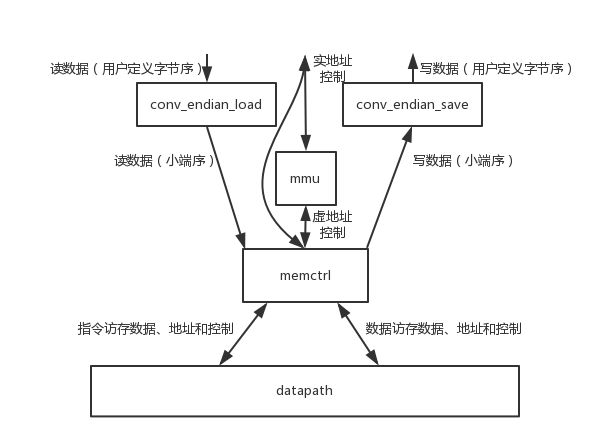
\includegraphics[width=.8\textwidth]{mem-data-flow.png}
	\caption{访存控制层数据/控制流}
    \label{fig:mem-data-flow}
\end{figure}

\subsection{各实体说明}

以下介绍除访存控制层除顶层实体外的各实体。顶层实体cpu的说明见上层(I/O层)。

\subsubsection{datapath}

\paragraph{功能}\mbox{}

数据通路层顶层实体(详细说明见本文数据通路层一节)。

\paragraph{参数}\mbox{}

datapath实体的参数定义见Table~\ref{tb:datapath-parameter}。
\begin{table}[!htb]
\begin{center}
\begin{tabular*}{15cm}{l|l|l}
\hline
\textbf{参数}&\textbf{类型}&\textbf{功能} \\
\hline instEntranceAddr        & std\_logic\_vector(AddrWidth)    & 重置后PC的值 \\
\hline exceptBootBaseAddr      & std\_logic\_vector(AddrWidth)    & 启动时异常处理向量的基地址 \\
\hline tlbRefillExl0Offset     & std\_logic\_vector(AddrWidth)    & 异常态下TLB缺失异常的偏移量 \\
\hline generalExceptOffset     & std\_logic\_vector(AddrWidth)    & 一般的异常处理向量的基地址 \\
\hline interruptIv1Offset      & std\_logic\_vector(AddrWidth)    & $Cause_{IV}=1$时的中断异常偏移量 \\
\hline
\end{tabular*}
\caption{datapath实体的参数}
\label{tb:datapath-parameter}
\end{center}
\end{table}

\paragraph{接口}\mbox{}

datapath实体的接口定义见Table~\ref{tb:datapath-interface}。
\begin{longtable}{l|l|l|l|p{5cm}}
\hline
\textbf{信号}&\textbf{宽度}&\textbf{I/O}&\textbf{来源/去向}&\textbf{功能} \\
\hline \endhead rst            & 1                      & I     & 上层          & 同步重置 \\
\hline clk                     & 1                      & I     & 上层          & 时钟 \\
\hline instData\_i             & InstWidth              & I     & memctrl       & 指令读数据 \\
\hline instAddr\_o             & AddrWidth              & O     & memctrl       & 指令读地址 \\
\hline instEnable\_o           & 1                      & O     & memctrl       & 指令读使能 \\
\hline dataData\_i             & DataWidth              & I     & memctrl       & 数据读数据 \\
\hline dataData\_o             & DataWidth              & O     & memctrl       & 数据写数据 \\
\hline dataAddr\_o             & AddrWidth              & O     & memctrl       & 数据读/写地址 \\
\hline dataEnable\_o           & 1                      & O     & memctrl       & 数据访存使能 \\
\hline dataWrite\_o            & 1                      & O     & memctrl       & 数据写使能 \\
\hline dataByteSelect\_o       & 3..0                   & O     & memctrl       & 数据字节选择 \\
\hline instExcept\_i           & ExceptionCauseWidth    & I     & memctrl       & 指令访存异常 \\
\hline dataExcept\_i           & ExceptionCauseWidth    & I     & memctrl       & 数据访存异常 \\
\hline ifToStall\_i            & 1                      & I     & memctrl       & 指令访存暂停 \\
\hline memToStall\_i           & 1                      & I     & memctrl       & 数据访存暂停 \\
\hline int\_i                  & IntWidth               & I     & 上层          & 外设中断 \\
\hline timerInt\_o             & 1                      & O     & 上层          & 时钟中断 \\
\hline isKernelMode\_o         & 1                      & O     & mmu           & 高电平表示当前处于内核态 \\
\hline entryWrite\_o           & 1                      & O     & mmu           & TLB写使能 \\
\hline entryIndex\_o           & TLBIndexWidth          & O     & mmu           & 要写的TLB表项索引 \\
\hline entry\_o                & 3*32(复合类型)         & O     & mmu           & 要写的TLB表项内容 \\
\hline
\caption{datapath实体的接口}
\label{tb:datapath-interface}
\end{longtable}

\subsubsection{memctrl}

\paragraph{功能}\mbox{}

处理指令访存(取指)和数据访存之间的结构冲突。

\paragraph{接口}\mbox{}

memctrl实体的接口定义见Table~\ref{tb:memctrl-interface}。
\begin{longtable}{l|l|l|l|p{5cm}}
\hline
\textbf{信号}&\textbf{宽度}&\textbf{I/O}&\textbf{来源/去向}&\textbf{功能} \\
\hline \endhead instData\_o    & InstWidth              & O     & datapath      & 指令读数据 \\
\hline instAddr\_i             & AddrWidth              & I     & datapath      & 指令读地址 \\
\hline instEnable\_i           & 1                      & I     & datapath      & 指令读使能 \\
\hline instStall\_o            & 1                      & O     & datapath      & 指令访存暂停 \\
\hline instExcept\_o           & ExceptionCauseWidth    & O     & datapath      & 指令访存异常 \\
\hline dataData\_o             & DataWidth              & O     & datapath      & 数据读数据 \\
\hline dataData\_i             & DataWidth              & I     & datapath      & 数据写数据 \\
\hline dataAddr\_i             & AddrWidth              & I     & datapath      & 数据读/写地址 \\
\hline dataEnable\_i           & 1                      & I     & datapath      & 数据访存使能 \\
\hline dataWrite\_i            & 1                      & I     & datapath      & 数据写使能 \\
\hline dataByteSelect\_i       & 3..0                   & I     & datapath      & 数据字节选择 \\
\hline dataStall\_i            & 1                      & O     & datapath      & 数据访存暂停 \\
\hline dataExcept\_o           & ExceptionCauseWidth    & O     & datapath      & 数据访存异常 \\
\hline devData\_i              & DataWidth              & I     & conv\_endian\_load & 统一访存读数据 \\
\hline devData\_o              & DataWidth              & O     & conv\_endian\_save & 统一访存写数据 \\
\hline devAddr\_o              & AddrWidth              & O     & mmu           & 统一访存读/写地址 \\
\hline devEnable\_o            & 1                      & O     & mmu           & 统一访存使能 \\
\hline devWrite\_o             & 1                      & O     & 上层          & 统一访存写使能 \\
\hline devByteSelect\_o        & 3..0                   & O     & 上层          & 统一访存字节选择 \\
\hline devBusy\_i              & 1                      & I     & 上层          & 统一访存暂停 \\
\hline devExcept\_i            & ExceptionCauseWidth    & I     & mmu           & 统一访存异常 \\
\hline
\caption{memctrl实体的接口}
\label{tb:memctrl-interface}
\end{longtable}

\paragraph{设计}\mbox{}

memctrl是组合逻辑电路,与时钟无关。

处理指令访存与数据访存的结构冲突时,数据访存的优先级更高。因为如果反过来,优先进行指令访存,而暂停了流水线的访存阶段(数据访存),其之前的取指阶段(指令访存)也会被暂停,导致两种访存都无法进行。因此,memctrl实体的逻辑如下:

\begin{enumerate}
    \item 当数据访存被使能时,向datapath发出暂停流水线取指阶段(插入空泡)的请求,将去往/来自上层的数据访存的信号与去往/来自下层的统一访存信号相连,忽略指令访存使能信号;
    \item 否则,当指令访存被使能时,将去往/来自上层的指令访存的信号与去往/来自下层的统一访存信号相连,并补充指令访存省略的相关控制信号,例如写使能为低电平。
\end{enumerate}

从上述逻辑可以看出,memctrl本质上是一个二选一选择器。

\subsubsection{mmu}

\paragraph{功能}\mbox{}

mmu实体根据MIPS32的地址映射方案,对不同地址分别使用直接偏移或查找TLB的方式进行翻译,并识别非法地址。mmu实体还负责TLB表项的维护工作。

\paragraph{接口}\mbox{}

mmu实体的接口定义见Table~\ref{tb:mmu-interface}。
\begin{table}[!htb]
\begin{center}
\begin{tabular*}{15cm}{l|l|l|l|p{5cm}}
\hline
\textbf{信号}&\textbf{宽度}&\textbf{I/O}&\textbf{来源/去向}&\textbf{功能} \\
\hline rst                     & 1                      & I     & 上层          & 同步重置 \\
\hline clk                     & 1                      & I     & 上层          & 时钟 \\
\hline enable\_i               & 1                      & I     & memctrl       & 使能 \\
\hline enable\_o               & 1                      & O     & 上层          & 使能 \\
\hline isLoad\_i               & 1                      & I     & memctrl       & 读使能,即$\overline{\text{写使能}}$ \\
\hline isKernelMode\_i         & 1                      & I     & memctrl       & 高电平表示当前处于内核态 \\
\hline addr\_i                 & AddrWidth              & I     & memctrl       & 虚地址 \\
\hline addr\_o                 & AddrWidth              & O     & 上层          & 实地址 \\
\hline entryWrite\_i           & 1                      & I     & memctrl       & TLB写使能 \\
\hline index\_i                & TLBIndexWidth          & I     & memctrl       & 要写的TLB表项索引 \\
\hline entry\_i                & 3*32(复合类型)         & I     & memctrl       & 要写的TLB表项内容 \\
\hline exceptCause\_o          & ExceptionCauseWidth    & O     & memctrl       & 异常类型或无异常 \\
\hline
\end{tabular*}
\caption{mmu实体的接口}
\label{tb:mmu-interface}
\end{center}
\end{table}

\paragraph{设计}\mbox{}

MIPS32规定的地址映射方案如Table~\ref{tb:mem-map}。由于nCore没有实现缓存,故可省略缓存相关约定。
\begin{table}[!htb]
\begin{center}
\begin{tabular*}{15cm}{l|l|l|l}
\hline
\textbf{段}&\textbf{虚拟地址(VA)}&\textbf{权限}&\textbf{物理地址(PA)} \\
\hline kuseg & 0x00000000 - 0x7FFFFFFF & 用户态 & TLB \\
\hline kseg0 & 0x80000000 - 0x9FFFFFFF & 内核态 & 0x00000000 - 0x1FFFFFFF \\
\hline kseg1 & 0xA0000000 - 0xBFFFFFFF & 内核态 & 0x00000000 - 0x1FFFFFFF \\
\hline kseg2 & 0xC0000000 - 0xFFFFFFFF & 内核态 & TLB \\
\hline
\end{tabular*}
\caption{地址映射方案}
\label{tb:mem-map}
\end{center}
\end{table}

根据地址映射方案,mmu实体翻译地址的过程如下。翻译过程由组合逻辑实现,与时钟无关。

\begin{enumerate}
    \item 大于等于0x80000000的地址需要内核态才能访问,若不是内核态,则产生读/写地址异常。
    \item 若虚地址落在kseg0段,直接减去0x80000000的偏移量即完成翻译。
    \item 若虚地址落在kseg1段,直接减去0xA0000000的偏移量即完成翻译。
    \item 否则需要使用TLB进行翻译,过程如下
    \begin{enumerate}
        \item mmu实体实现了16路全相联的TLB。MIPS32在不做配置的情况下,每页内存大小为4KB,故地址的高20位为页号,低12位为页内偏移量。MIPS32规定虚地址空间中连续的两个虚页共用同一个TLB表项,故应在所有16项中找出虚地址的高19位与表项中记载的相符的那一项。
        \item 对于找出的这一项,当且仅当其ASID(地址空间标识符)域与当前CP0中记载相符,或其中两个实页的G(全局)位均为1时,此项才有效。
        \item 在找出的TLB表项的两个实页中找出对应的一页,当且仅当该页的V(有效)位为1时,此页才有效。
        \item 最后,还需检查该实页的D(脏)位,若D位为1则不能进行写操作。
    \end{enumerate}
    若以上任何一项不符,均产生读/写TLB缺失异常。
\end{enumerate}

按照MIPS32的约定,无论有效与否,TLB中是不会同时存在两个虚地址相同的页的,所以效率最高的查找方式是对TLB每一项进行不分先后的并行查找。一旦在某一项中找到了该虚页对应的实页,就将该实页号输出到一个总线上。然而,由于无法在FPGA芯片内实现三态逻辑,即无法实现上述总线,只能进行有先后次序的查找。尽管如此,查找过程依然是一个组合逻辑过程,VHDL综合器会将其视作一个整体进行优化,逻辑的许多部分依然是并行执行的,故不会造成显著的性能损失。

此外还有一点值得注意:目标程序\textmu Core可能违反上述约定,即\textmu Core可能向不同的TLB表项写入相同地址的虚页。因此,当在TLB中查询到某一个虚页并发现其无效时,不能放弃查询。必须检查完所有的表项后,才能确定是否发生了TLB缺失。

mmu实体还负责TLB的维护工作,即向TLB表项中写入新值。此情形下,TLB与寄存器堆无异,只需在时钟上升沿处将表项值更新为输入值即可(写入操作为时序逻辑)。重置时,各表项置零。

\subsubsection{conv\_endian\_load、conv\_endian\_save}

\paragraph{功能}\mbox{}

实体conv\_endian\_load和conv\_endian\_save实现字节序转换,可通过参数使能。不使能时输出与输入相同。

这两个实体是同一个元件conv\_endian的例化,分别负责输入和输出两个方向的字节序转换,以下统一叙述。

\paragraph{参数}\mbox{}

conv\_endian元件的参数定义见Table~\ref{tb:convendian-parameter}。
\begin{table}[!htb]
\begin{center}
\begin{tabular*}{15cm}{l|l|l}
\hline
\textbf{参数}&\textbf{类型}&\textbf{功能} \\
\hline enable        & boolean    & 使能 \\
\hline
\end{tabular*}
\caption{conv\_endian元件的参数}
\label{tb:convendian-parameter}
\end{center}
\end{table}

\paragraph{接口}\mbox{}

conv\_endian元件的接口定义见Table~\ref{tb:convendian-interface}。
\begin{table}[!htb]
\begin{center}
\begin{tabular*}{15cm}{l|l|l|l|p{5cm}}
\hline
\textbf{信号}&\textbf{宽度}&\textbf{I/O}&\textbf{来源/去向}&\textbf{功能} \\
\hline input                   & DataWidth              & I     & memctrl(conv\_endian\_save), 上层(conv\_endian\_load)   & 输入 \\
\hline output                  & DataWidth              & O     & memctrl(conv\_endian\_load), 上层(conv\_endian\_save)   & 输出 \\
\hline
\end{tabular*}
\caption{conv\_endian元件的接口}
\label{tb:convendian-interface}
\end{center}
\end{table}

\paragraph{设计}\mbox{}

尽管nCore需要运行的目标程序都是小端序的,但在调试时构造一个大端序的仿真环境更为方便,因为这样可以将指令字原封不动地写入被仿真虚拟存储器里。实体conv\_endian\_load和conv\_endian\_save引入了编译期可选的字节序转换,为在不同的环境下运行或调试提供了便利。

\section{I/O层}

\subsection{概述}

本层将访存控制层提供的统一访存请求特化到不同的外设上。

本层包含的所有实体见Table~\ref{tb:io-entities}:

\begin{table}[!htb]
\begin{center}
\begin{tabular*}{15cm}{l|l}
\hline
\textbf{实体}&\textbf{功能} \\
\hline thinpad\_top & 顶层实体 \\
\hline cpu & 访存控制层 \\
\hline clk\_ctrl & 时钟驱动器 \\
\hline segL, segH & 七段数码管驱动器 \\
\hline devctrl & 多路选择器,用于将访存请求转发给各设备的驱动实体 \\
\hline base\_sram\_ctrl, ext\_sram\_ctrl & SRAM存储器驱动 \\
\hline flash\_ctrl & Flash存储器驱动 \\
\hline vga\_ctrl & 显示器驱动 \\
\hline serial\_ctrl & 串口驱动 \\
\hline async\_receiver & 串口接收器 \\
\hline async\_transmiter & 串口发送器 \\
\hline usb\_ctrl & USB驱动 \\
\hline boot\_ctrl & 启动用ROM驱动 \\
\hline lattice\_ram\_ctrl & 字体专用存储器驱动 \\
\hline eth\_ctrl & 以太网驱动 \\
\hline
\end{tabular*}
\caption{访存控制层的实体}
\label{tb:io-entities}
\end{center}
\end{table}

\subsection{整体设计}

在典型的计算机组成中,会使用总线连接各个设备驱动器。但是在nCore中,所有的设备驱动器均享有独立的FPGA芯片引脚,故只需实现一个多路选择器,从所有设备驱动器中选择一个连向cpu实体即可。这项工作由devctrl实体完成,它判断当前的访存地址落在哪个设备的地址段内,从而选择某一设备驱动器,即将数据和使能信号转发至该设备驱动器,或从该设备驱动器接收。

从逻辑上看,所有设备驱动器均是同一个基类的子类。虽然VHDL中并不能直接实现面向对象编程,但在nCore的实现中,除省略某些值为常量的接口外,所有设备驱动器都尽量统一了接口格式。

此外,并不是所有数据或控制信号都要由devctrl转发,由于使能信号以外的输入信号是不会对不使能的设备驱动器产生副作用的,所以地址信号和字节选择信号可以不加区分地发往所有设备。

I/O层的主要数据/控制流见Figure~\ref{fig:io-data-flow}。

\begin{figure}[!htb]
	\centering
	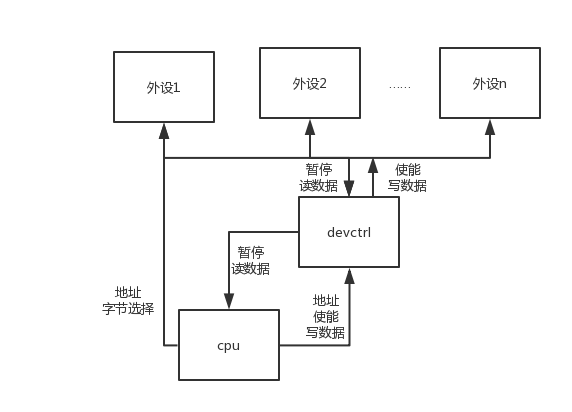
\includegraphics[width=.8\textwidth]{io-data-flow.png}
	\caption{I/O数据/控制流}
    \label{fig:io-data-flow}
\end{figure}

\subsection{各实体说明}

以下介绍除访存控制层除顶层实体外的各实体。顶层实体thinpad\_top的功能即本层功能,接口即本层所有来源/去向标为“外部”的接口,不再列表叙述。

\subsubsection{cpu}

\paragraph{功能}\mbox{}

cpu是访存控制层的顶层实体。具体说明请见本文访存控制层一节。

\paragraph{参数}\mbox{}

cpu实体的参数定义见Table~\ref{tb:cpu-parameter}。
\begin{table}[!htb]
\begin{center}
\begin{tabular*}{15cm}{l|l|l}
\hline
\textbf{参数}&\textbf{类型}&\textbf{功能} \\
\hline instEntranceAddr        & std\_logic\_vector(AddrWidth)    & 重置后PC的值 \\
\hline exceptBootBaseAddr      & std\_logic\_vector(AddrWidth)    & 启动时异常处理向量的基地址 \\
\hline tlbRefillExl0Offset     & std\_logic\_vector(AddrWidth)    & 异常态下TLB缺失异常的偏移量 \\
\hline generalExceptOffset     & std\_logic\_vector(AddrWidth)    & 一般的异常处理向量的基地址 \\
\hline interruptIv1Offset      & std\_logic\_vector(AddrWidth)    & $Cause_{IV}=1$时的中断异常偏移量 \\
\hline convEndianEnable        & boolean                          & 字节转换使能 \\
\hline
\end{tabular*}
\caption{cpu实体的参数}
\label{tb:cpu-parameter}
\end{center}
\end{table}

\paragraph{接口}\mbox{}

cpu实体的接口定义见Table~\ref{tb:cpu-interface}。
\begin{table}[!htb]
\begin{center}
\begin{tabular*}{15cm}{l|l|l|l|p{5cm}}
\hline
\textbf{信号}&\textbf{宽度}&\textbf{I/O}&\textbf{来源/去向}&\textbf{功能} \\
\hline rst                     & 1                      & I     & 外部          & 同步重置 \\
\hline clk                     & 1                      & I     & clk\_ctrl     & 时钟 \\
\hline devDataLoad\_i          & DataWidth              & I     & devctrl       & 访存读数据 \\
\hline devDataSave\_o          & DataWidth              & O     & devctrl       & 访存写数据 \\
\hline devPhysicalAddr\_o      & AddrWidth              & O     & devctrl、各设备驱动 & 访存读/写地址 \\
\hline devEnable\_o            & 1                      & O     & devctrl       & 访存使能 \\
\hline devWrite\_o             & 1                      & O     & devctrl       & 访存写使能 \\
\hline devByteSelect\_o        & 3..0                   & O     & 各设备驱动    & 访存字节选择 \\
\hline devBusy\_i              & 1                      & I     & devctrl       & 访存暂停 \\
\hline int\_i                  & IntWidth               & I     & cpu、外部     & 外设中断 \\
\hline timerInt\_o             & 1                      & O     & cpu           & 时钟中断 \\
\hline
\end{tabular*}
\caption{cpu实体的接口}
\label{tb:cpu-interface}
\end{center}
\end{table}

\subsubsection{clk\_ctrl}

\paragraph{功能}\mbox{}

clk\_ctrl是时钟驱动器,负责根据晶振产生的50MHz时钟信号生成nCore所需频率(目前是25MHz)的时钟信号。

clk\_ctrl逻辑上并不是I/O层的一部分,但由于所有时序逻辑实体都需要时钟,所以时钟驱动器必须至于最顶层实体处,即I/O层中。

\paragraph{接口}\mbox{}

clk\_ctrl实体的接口定义见Table~\ref{tb:clkctrl-interface}。
\begin{table}[!htb]
\begin{center}
\begin{tabular*}{15cm}{l|l|l|l|p{5cm}}
\hline
\textbf{信号}&\textbf{宽度}&\textbf{I/O}&\textbf{来源/去向}&\textbf{功能} \\
\hline clk\_in1                & 1                      & I     & 外部                  & 时钟输入 \\
\hline clk\_out1               & 1                      & O     & 各时序逻辑实体        & 时钟输出 \\
\hline
\end{tabular*}
\caption{clk\_ctrl实体的接口}
\label{tb:clkctrl-interface}
\end{center}
\end{table}

\paragraph{设计}\mbox{}

clk\_ctrl直接例化了Xilinx的IP核。

\subsubsection{segL, segH}

\paragraph{功能}\mbox{}

七段数码管驱动器(译码器)。segL和segH均例化了元件SEG7\_LUT,分别驱动实验电路板上的低位数字和高位数字。

\paragraph{接口}\mbox{}

SEG7\_LUT元件的接口定义见Table~\ref{tb:seg7lut-interface}。
\begin{table}[!htb]
\begin{center}
\begin{tabular*}{15cm}{l|l|l|l|p{5cm}}
\hline
\textbf{信号}&\textbf{宽度}&\textbf{I/O}&\textbf{来源/去向}&\textbf{功能} \\
\hline oSEG1                   & 7                      & O     & 外部                  & 译码输出 \\
\hline iDIG                    & 4                      & I     & devctrl             & 二进制输入 \\
\hline
\end{tabular*}
\caption{SEG7\_LUT元件}
\label{tb:seg7lut-interface}
\end{center}
\end{table}

\paragraph{设计}\mbox{}

元件SEG7\_LUT由课程提供。

\subsubsection{devctrl}

\paragraph{功能}\mbox{}

根据访存地址选择相应的设备驱动器,将cpu的数据和控制信号连接至该驱动器。

\paragraph{接口}\mbox{}

devctrl实体的接口定义见Table~\ref{tb:devctrl-interface}。
\begin{longtable}{l|l|l|l|p{5cm}}
\hline
\textbf{信号}&\textbf{宽度}&\textbf{I/O}&\textbf{来源/去向}&\textbf{功能} \\
\hline \endhead devEnable\_i   & 1                      & I     & cpu               & 统一访存使能 \\
\hline devWrite\_i             & 1                      & I     & cpu               & 统一访存写使能 \\
\hline devBusy\_o              & 1                      & O     & cpu               & 统一访存暂停 \\
\hline devDataSave\_i          & DataWidth              & I     & cpu               & 统一访存写数据 \\
\hline devDataLoad\_o          & DataWidth              & O     & cpu               & 统一访存读数据 \\
\hline devPhysicalAddr\_i      & AddrWidth              & I     & cpu               & 统一访存读/写地址 \\
\hline ram0Enable\_o           & 1                      & O     & base\_sram\_ctrl  & SRAM0使能 \\
\hline ram0ReadEnable\_o       & 1                      & O     & base\_sram\_ctrl  & SRAM0读使能,即$\overline{\text{写使能}}$ \\
\hline ram0DataSave\_o         & DataWidth              & O     & base\_sram\_ctrl  & SRAM0写数据 \\
\hline ram0DataLoad\_i         & DataWidth              & I     & base\_sram\_ctrl  & SRAM0读数据 \\
\hline ram0WriteBusy\_i        & 1                      & I     & base\_sram\_ctrl  & SRAM0暂停 \\
\hline ram1Enable\_o           & 1                      & O     & ext\_sram\_ctrl   & SRAM1使能 \\
\hline ram1ReadEnable\_o       & 1                      & O     & ext\_sram\_ctrl   & SRAM1读使能,即$\overline{\text{写使能}}$ \\
\hline ram1DataSave\_o         & DataWidth              & O     & ext\_sram\_ctrl   & SRAM1写数据 \\
\hline ram1DataLoad\_i         & DataWidth              & I     & ext\_sram\_ctrl   & SRAM1读数据 \\
\hline ram1WriteBusy\_i        & 1                      & I     & ext\_sram\_ctrl   & SRAM1暂停 \\
\hline flashEnable\_o          & 1                      & O     & flash\_ctrl       & Flash使能 \\
\hline flashReadEnable\_o      & 1                      & O     & flash\_ctrl       & Flash读使能,即$\overline{\text{写使能}}$ \\
\hline flashDataLoad\_i        & DataWidth              & I     & flash\_ctrl       & Flash读数据 \\
\hline flashBusy\_i            & 1                      & I     & flash\_ctrl       & Flash暂停 \\
\hline vgaEnable\_o            & 1                      & O     & vga\_ctrl         & 显示器使能 \\
\hline vgaWriteEnable\_o       & 1                      & O     & vga\_ctrl         & 显示器写使能 \\
\hline vgaWriteData\_o         & DataWidth              & O     & vga\_ctrl         & 显示器写数据 \\
\hline comEnable\_o            & 1                      & O     & serial\_ctrl      & 串口使能 \\
\hline comReadEnable\_o        & 1                      & O     & serial\_ctrl      & 串口读使能,即$\overline{\text{写使能}}$ \\
\hline comDataSave\_o          & DataWidth              & O     & serial\_ctrl      & 串口写数据 \\
\hline comDataLoad\_i          & DataWidth              & I     & serial\_ctrl      & 串口读数据 \\
\hline usbEnable\_o            & 1                      & O     & usb\_ctrl         & USB使能 \\
\hline usbReadEnable\_o        & 1                      & O     & usb\_ctrl         & USB读使能 \\
\hline usbReadData\_i          & DataWidth              & I     & usb\_ctrl         & USB读数据 \\
\hline usbWriteEnable\_o       & 1                      & O     & usb\_ctrl         & USB写使能 \\
\hline usbWriteData\_o         & DataWidth              & O     & usb\_ctrl         & USB写数据 \\
\hline usbBusy\_i              & 1                      & I     & usb\_ctrl         & USB暂停 \\
\hline bootDataLoad\_i         & DataWidth              & I     & boot\_ctrl        & 启动用ROM读数据 \\
\hline ltcEnable\_o            & 1                      & O     & lattice\_ram\_ctrl& 点阵(字体)存储器使能 \\
\hline ltcReadEnable\_o        & 1                      & O     & lattice\_ram\_ctrl& 点阵(字体)存储器读使能,即$\overline{\text{写使能}}$ \\
\hline ltcDataLoad\_i          & DataWidth              & I     & lattice\_ram\_ctrl& 点阵(字体)存储器读数据 \\
\hline ltcBusy\_i              & 1                      & I     & lattice\_ram\_ctrl& 点阵(字体)存储器暂停 \\
\hline ethEnable\_o            & 1                      & O     & eth\_ctrl         & 以太网使能 \\
\hline ethReadEnable\_o        & 1                      & O     & eth\_ctrl         & 以太网读使能,即$\overline{\text{写使能}}$ \\
\hline ethDataSave\_o          & DataWidth              & O     & eth\_ctrl         & 以太网写数据 \\
\hline ethDataLoad\_i          & DataWidth              & I     & eth\_ctrl         & 以太网读数据 \\
\hline ethWriteBusy\_i         & 1                      & I     & eth\_ctrl         & 以太网暂停 \\
\hline ledEnable\_o            & 1                      & O     & 外部              & LED使能 \\
\hline ledData\_o              & DataWidth              & O     & 外部              & LED写数据 \\
\hline numEnable\_o            & 1                      & O     & segL、segH        & 七段数码管使能 \\
\hline numData\_o              & DataWidth              & O     & segL、segH        & 七段数码管写数据 \\
\hline
\caption{devctrl实体的接口}
\label{tb:devctrl-interface}
\end{longtable}

\paragraph{设计}\mbox{}

各设备的地址段分配见Table~\ref{tb:dev-addr},devctrl按此规则选择即可。部分设备是只读或只写的,则相应写或读的信号可以省略;部分设备是不会请求暂停的,故暂停信号可以省略。
\begin{table}[!htb]
\begin{center}
\begin{tabular}{p{7.5cm}|p{7.5cm}}
\hline
\textbf{设备}&\textbf{地址段} \\
\hline RAM0             & 0x00000000 - 0x003FFFFF \\
\hline RAM1             & 0x00400000 - 0x007FFFFF \\
\hline Flash            & 0x1E000000 - 0x1EFFFFFF \\
\hline 启动用ROM        & 0x1FC00000 - 0x1FC00FFF \\
\hline 串口             & 0x1FD003F8 - 0x1FD003FC \\
\hline LED              & 0x1FD0F000 \\
\hline 七段数码管       & 0x1FD0F010 \\
\hline 显示器           & 0x1FE00000 - 0x1FE4AFFF \\
\hline 点阵(字体)存储器&0x1FE4B000 - 0x1FE4B7FF \\
\hline 以太网           & 0x1C020100 - 0x1C020104 \\
\hline USB              & 0x1C020000 - 0x1C020004 \\
\hline
\end{tabular}
\caption{外设地址分配}
\label{tb:dev-addr}
\end{center}
\end{table}

\subsubsection{base\_sram\_ctrl, ext\_sram\_ctrl}

\paragraph{功能}\mbox{}

base\_sram\_ctrl和ext\_sram\_ctrl均例化了元件sram\_ctrl,分别SRAM0与SRAM1存储器的控制器。

\paragraph{接口}\mbox{}

sram\_ctrl元件的接口定义见Table~\ref{tb:sramctrl-interface}。
\begin{table}[!htb]
\begin{center}
\begin{tabular*}{15cm}{l|l|l|l|p{5cm}}
\hline
\textbf{信号}&\textbf{宽度}&\textbf{I/O}&\textbf{来源/去向}&\textbf{功能} \\
\hline rst                     & 1                      & I     & 外部          & 同步重置 \\
\hline clk                     & 1                      & I     & clk\_ctrl     & 时钟 \\
\hline enable\_i               & 1                      & I     & devctrl       & 使能 \\
\hline readEnable\_i           & 1                      & I     & devctrl       & 读使能,即$\overline{\text{写使能}}$ \\
\hline addr\_i                 & AddrWidth              & I     & cpu           & 地址 \\
\hline byteSelect\_i           & 3..0                   & I     & cpu           & 字节选择 \\
\hline busy\_o                 & 1                      & O     & devctrl       & 暂停请求 \\
\hline triStateWrite\_o        & 1                      & O     & N/A(下文详述)&高电平表示应向三态总线上写 \\
\hline addr\_o                 & 19..0                  & O     & 外部          & 芯片地址(按字编制) \\
\hline be\_n\_o                & 3..0                   & O     & 外部          & 芯片$\overline{\text{字节选择}}$ \\
\hline ce\_n\_o                & 1                      & O     & 外部          & 芯片$\overline{\text{使能}}$ \\
\hline oe\_n\_o                & 1                      & O     & 外部          & 芯片$\overline{\text{读使能}}$ \\
\hline we\_n\_o                & 1                      & O     & 外部          & 芯片$\overline{\text{写使能}}$ \\
\hline
\end{tabular*}
\caption{sram\_ctrl元件}
\label{tb:sramctrl-interface}
\end{center}
\end{table}

\paragraph{设计}\mbox{}

实验电路板上的SRAM芯片是异步的,这意味着随时可以通过组合逻辑的方式读而不需等待时钟。但这样并不意味着随时可写,随时写入可能会导致两类错误:

\begin{enumerate}
    \item 若写使能刚刚被置就立即写入,可能由于地址还未被稳定地计算出来,导致破坏其他存储单元;
    \item 若写入完成后,写使能信号比数据和地址还晚撤出,可能破坏已写入的数据,也可能破坏其他存储单元。
\end{enumerate}

\begin{figure}[!htb]
	\centering
	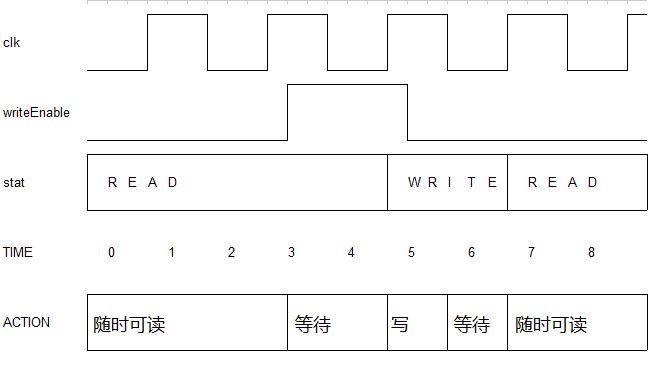
\includegraphics[width=.8\textwidth]{sram-ctrl.png}
	\caption{SRAM时序}
    \label{fig:sram-ctrl}
\end{figure}

为了解决以上问题,sram\_ctrl中为写入操作设计了一个简单的状态机。以Figure~\ref{fig:sram-ctrl}为例:$writeEnable$表示写使能;$stat$表示状态,可能取值为$READ$或$WRITE$。若$stat=READ$且$writeEnable=0$,例如$0 \le TIME \le 2$时,则随时可读。

$TIME=3$时$writeEnable$被置为1,此时不再可读,但出于上述第1点原因,并不能立即写入,sram\_ctrl会向cpu发出暂停信号,使此写请求保持到写一个周期。当下一个时钟上升沿到来时,$stat$被置为$WRITE$,此时芯片的写使能才被置,进行写操作。然而,又出于上述第二点原因,只有$stat=WRITE$且$clk=1$时芯片的写使能才被置。也就是说,芯片的写使能会提早半个周期撤出。所以只有$TIME=5$时可以进行写操作,而$TIME=6$时不可以。

当下一个上升沿来临时,即$TIME=7$时,写操作全部完成,$stat$恢复为$READ$,SRAM重新进入随时可读的状态。

SRAM读写的另一个问题是三态信号的使用。进行读操作时,外设向信号写入,sram\_ctrl读;进行写操作时,sram\_ctrl向信号写入,外设读。应确保不会有两个主体同时向三态信号写入,以免发生短路。三态信号的读写也应避免上述的两点时序错误,分析可知,sram\_ctrl应在$stat=WRITE$时写三态信号,其余时间读或忽略。

由于FPGA中只有I/O模块具有操作三态信号的能力,使用VHDL开发时不建议在非顶层实体中使用三态信号,以免综合器将其视为普通信号却难以发现。所以sram\_ctrl并没有直接操作三态信号,而是输出triStateWrite\_o控制信号,表明应向三态信号写,还是从三态信号读。对三态信号的直接操作在thinpad\_top实体中完成。

\subsubsection{flash\_ctrl}
\subsubsection{vga\_ctrl}
\subsubsection{serial\_ctrl}
\subsubsection{async\_receiver}
\subsubsection{async\_transmiter}
\subsubsection{usb\_ctrl}
\subsubsection{boot\_ctrl}
\subsubsection{lattice\_ram\_ctrl}
\subsubsection{eth\_ctrl}

%%%%%%%%%%%%%%%%%%%%%%
%     BODY END       %
%%%%%%%%%%%%%%%%%%%%%%

\end{spacing}
\end{document}